% Assembled from main.tex and article/*.tex.
% Rebuild with python code/build_article.py.

% BEGIN article/preamble.tex
\documentclass[11pt,a4paper]{article}
\usepackage[T1]{fontenc}
\usepackage[utf8]{inputenc}
\usepackage{lmodern}
\usepackage[margin=24mm,headheight=14pt]{geometry}
\usepackage{amsmath,amssymb,amsthm,mathtools,mathrsfs}
\usepackage{microtype}
\usepackage{booktabs,longtable,array,tabularx}
\usepackage{graphicx,xcolor}
\usepackage{enumitem}
\usepackage{fancyhdr}
\usepackage{url}
\usepackage[unicode,pdfencoding=auto,psdextra]{hyperref}
\usepackage[nameinlink,noabbrev]{cleveref}
\definecolor{inkblue}{HTML}{183D59}
\hypersetup{colorlinks=true,linkcolor=inkblue,citecolor=inkblue,urlcolor=inkblue,
 pdftitle={Further Identities and Critical Transitions in the Polylogarithm--Stieltjes Calculus},
 pdfauthor={Research continuation prepared for Vladimir Reshetnikov}}
\numberwithin{equation}{section}
\newtheorem{theorem}{Theorem}[section]
\newtheorem{lemma}[theorem]{Lemma}
\newtheorem{proposition}[theorem]{Proposition}
\newtheorem{corollary}[theorem]{Corollary}
\newtheorem{conjecture}[theorem]{Conjecture}
\theoremstyle{definition}
\newtheorem{definition}[theorem]{Definition}
\newtheorem{question}[theorem]{Question}
\theoremstyle{remark}
\newtheorem{remark}[theorem]{Remark}
\newtheorem{example}[theorem]{Example}
\DeclareMathOperator{\Li}{Li}
\DeclareMathOperator{\sgn}{sgn}
\DeclareMathOperator{\Sh}{Sh}
\DeclareMathOperator{\Sym}{Sym}
\DeclareMathOperator{\im}{im}
\DeclareMathOperator{\tr}{tr}
\DeclareMathOperator{\ad}{ad}
\DeclareMathOperator{\depth}{depth}
\DeclareMathOperator{\rank}{rank}
\DeclareMathOperator{\Hilb}{Hilb}
\newcommand{\Q}{\mathbb Q}
\newcommand{\R}{\mathbb R}
\newcommand{\C}{\mathbb C}
\newcommand{\N}{\mathbb N}
\newcommand{\Z}{\mathbb Z}
\newcommand{\sh}{\mathbin{\shuffle}}
\newcommand{\shuffle}{\mathbin{\amalg}}
\newcommand{\repo}{\textsc{ProveIt}}
\newcommand{\baselinecommit}{570b0567f311cf1890865065896be2665f469e4f}
\newcolumntype{Y}{>{\raggedright\arraybackslash}X}
\setlist{itemsep=3pt,topsep=5pt,leftmargin=*}
\setlength{\emergencystretch}{1.5em}
\setlength{\parskip}{3pt plus 1pt}
\allowdisplaybreaks[1]
\pagestyle{fancy}
\fancyhf{}
\fancyhead[L]{\small Polylogarithm--Stieltjes research continuation}
\fancyhead[R]{\small October 2026}
\fancyfoot[C]{\thepage}
\renewcommand{\headrulewidth}{0.3pt}
\title{\textbf{Further Identities and Critical Transitions\\
in the Polylogarithm--Stieltjes Calculus}\\[7pt]
\large Translation geometry, Euler reversal, Lerch velocities,\\
and depth in the Cayley shuffle quotient}
\author{Research continuation prepared for Vladimir Reshetnikov\\
\normalsize For integration into the \repo\ project}
\date{10 October 2026}

% END article/preamble.tex

\begin{document}
\maketitle
\begin{abstract}
We continue the polylogarithm--Stieltjes program at a pinned ProveIt
repository snapshot. A holomorphic translation identity for Hurwitz zeta
generates all-order pairings of balanced Stieltjes antiderivatives,
explicit logarithmic endpoint polynomials, a positive Gram kernel,
and sharp Sobolev thresholds. Its first spectral derivative yields
three exact formulas for the periodic Gamma translation energy,
strict concavity with a unique half-period maximum, and a geometrically
convergent odd-zeta identity for the first Stieltjes constant.
An explicit epsilon-sensitive density estimate proves the existing
near-critical Euler reversal conjecture, with a first logarithmic
correction, Lambert approximation, derivative-zero ratios, and a
universal transition profile. For diagonal Lerch velocities we determine
the least eventual sign-block length and all-order sharp-cutoff finite
parts, including the essential conjugate-singularity terms.
Finally, an oriented shuffle-algebra retraction for the full Cayley ideal
preserves depth and gives exact filtered dimensions. The mixed $S_6$
and current $S_8$ period candidates remain conjectural. Proofs, explicit
source-status decisions, reproducible algebra and numerical diagnostics,
and a proposed research agenda accompany the article.
\end{abstract}
\vspace{4pt}
\noindent\textbf{Keywords.} Polylogarithm; Hurwitz zeta; Gamma function;
polygamma; generalized Stieltjes constants; Euler transformation;
Lambert inverse; shuffle algebra; critical asymptotics.
\clearpage
{\small\setlength{\parskip}{0pt}\tableofcontents}
\clearpage

% BEGIN article/00_introduction.tex
\section{Scope, principal results, and relation to the source material}
\label{sec:scope}

This report continues the polylogarithm manuscript and the active incoming
research of the \repo\ project. It is based on the fixed repository commit
\begin{center}\small\texttt{\baselinecommit}\end{center}
The consolidated manuscript and the newer
continuation reports must be read together: several questions still visible
in older fragments have already been settled in later reports. The source
comparison, exact paths, and proposed integration actions are supplied in
the accompanying claim ledger and provenance manifest.

The results here fall into four connected developments. The first is a
translation calculus for the Hurwitz order jets that generate balanced
Stieltjes antiderivatives. The second resolves an explicit joint-limit
conjecture for Gaussian polylogarithmic Euler remainders. The third studies
the exact signs and critical sums of the Lerch deformation velocities
already identified in the latest continuation. The fourth gives an
algebraic reduction preserving depth in the formal Cayley quotient.
Each development has its own hypotheses; none is used as a substitute for
an unproved arithmetic relation among numerical periods.

\subsection{Results at a glance}

\begin{enumerate}
\item \textbf{Exact translated Hurwitz pairings.}
Theorem~\ref{thm:translation} expresses the bilinear periodic translation
of two Hurwitz functions as a Gamma--trigonometric kernel times a
symmetric Hurwitz difference. Its polylogarithmic form permits every
order derivative. Theorem~\ref{thm:cusp} identifies the complete
logarithmic endpoint polynomial and an ordinary convergent even power
series remainder at every derivative order.

\item \textbf{A sharp Gamma translation inequality.}
The squared $L^2$ change in $\log\Gamma$ under a periodic translation is
strictly concave on $(0,1)$ and has its unique maximum at $1/2$
(Theorem~\ref{thm:gamma-max}). Its three exact representations yield
an accelerated odd-zeta series for $\gamma_1$ with an explicit geometric
tail (Corollary~\ref{cor:gamma1-fast}). Higher derivatives connect this
energy to polygamma functions and Hurwitz order derivatives; explicit
primitives follow from the same kernel.

\item \textbf{Proof of the near-critical Euler conjecture.}
For outer order $a=1-\varepsilon$, fixed inner order $b>0$, and
$\lambda=\log(1/\varepsilon)$, the unique reversal index satisfies
\[
 \nu(1-\varepsilon,b)\sim
 \frac{\lambda^{2b+2}}
 {\pi b^2\Gamma(b+1)^2\zeta(b+1)^2\varepsilon^2}.
\]
Theorem~\ref{eutrans:thm:crossing} proves the source conjecture
\texttt{research:conj:crossing}, including a first inverse-logarithmic
correction uniformly for $b$ in compact positive intervals. The proof
retains the exponentially small seed and an $\varepsilon$ factor in
the algebraic remainder. A rescaled profile is
$x^{-1/2}-x^{-1}$; the later maximum occurs at an index asymptotic
to $4\nu$.

\item \textbf{Optimal sign blocks and all-order critical finite parts.}
For the Lerch velocities $v_n(A)$, let $\theta(A)$ be the phase of
the dominant inverse singularity. The least eventual block length
containing both signs is exactly $\lceil\pi/\theta\rceil+1$
(Theorem~\ref{newdiag:thm:sharp-block}). At $A=2$ it is four.
Theorem~\ref{newdiag:thm:finiteparts} computes the finite part of every
sharp sum $\sum_{n\leq N}n^pv_n(A)\tau^n$. Both conjugate singularities
are required for the divergent subtractions once $p\geq2$.

\item \textbf{A depth-preserving formal Cayley reduction.}
An oriented choice of shuffle generators yields a multiplicative
retraction whose kernel is the full Cayley ideal and whose output
does not increase depth. Its generator counts give the exact depth
filtration of the quotient. This is a structural algebraic result;
the mixed $S_6$ period identity remains conjectural.
\end{enumerate}

\subsection{Classical antecedents and what is claimed here}

Hurwitz's Fourier expansion, the parameter recurrence, and the
order-zero Gamma evaluation are classical \cite{DLMFHurwitz}.
Espinosa and Moll developed product integrals and antiderivatives involving
Hurwitz zeta \cite{EM1,EM2}, and a generalized polygamma framework
\cite{EMPoly}. These works supply the appropriate context for the first
two sections. We give a direct analytic derivation of the translated
identities and their sharp consequences; the underlying unshifted product
integral is explicitly credited. The standard polylogarithm conventions
are those summarized in \cite{DLMFPolylog}.

The Euler section uses the exact density and the global one-crossing
theorem already proved in the newest applicable source \cite{RepoEuler}.
Its new work is the uniform estimate in the singular joint limit, the
corrected root law, and the profile consequences. The Lerch sections use
the selected-sheet continuation and additive coefficient asymptotic from
\cite{RepoLerch}; they answer two further questions posed there. Lagrange
inversion and singularity transfer are standard tools
\cite{Gessel,FlajoletOdlyzko}. Earlier Lambert polynomial and branch
expansions provide further context \cite{KaluginJeffrey,Cohen}.

Throughout, ``new'' means established here relative to the checked
repository baseline. This source audit is not a claim of worldwide
priority for every identity or special case. The classical tools are
identified, inherited repository theorems are marked, and new assertions
are supplied with proofs. The unresolved $S_6$ and current $S_8$ candidates
retain their conjectural status even when numerical residuals are tiny.

\subsection{Conventions and logical boundaries}

The Laurent convention is
$\zeta(1+u,a)=u^{-1}+\sum_{n\geq0}(-1)^n\gamma_n(a)u^n/n!$;
in particular $\gamma_0(a)=-\psi(a)$. Superscripts on $\zeta$ denote
derivatives with respect to its order, while superscripts on
$\gamma_n$ and $\psi$ denote derivatives with respect to their real
argument. Rising factorials are $(z)_m$ and falling factorials are
$(z)_{\underline m}$. Endpoint values of periodic $L^2$ functions are
understood almost everywhere. Branches of complex powers and square
roots are fixed where first used.

The analytic arguments, exact rational algebra, and floating-point
diagnostics play different roles. Proofs justify every limiting operation
that enters a theorem. Exact finite calculations check implementations
and stated ranks in specified spaces. Floating-point calculations test
formulas independently and illustrate asymptotic accuracy; they are not
interval certificates. The package does not claim proof-assistant
formalization or arithmetic independence from numerical experiments.

% END article/00_introduction.tex


% BEGIN article/01_translation.tex
\section{A translation calculus for Hurwitz jets}
\label{sec:translation}

The parameter identity $\partial_x\zeta(s,x)=-s\zeta(s+1,x)$
connects the three central objects of this section: Hurwitz order derivatives,
Stieltjes antiderivatives, and the logarithm of the Gamma function.
We add translation in $x$ as a second operation. The resulting bilinear
identity has both a polylogarithmic form and a Hurwitz form. The latter
makes all endpoint logarithms and all derivative orders explicit.

\subsection{Normalization and analytic justification}

Write
\begin{equation}\label{eq:stieltjes-def}
 \zeta(1+u,x)=\frac1u+\sum_{n=0}^{\infty}
              \frac{(-1)^n}{n!}\gamma_n(x)u^n,
 \qquad x>0.
\end{equation}
Order derivatives of $\zeta$ always refer to its first argument. Define
\begin{equation}\label{eq:FJ}
 F_r(x)=\zeta^{(r)}(0,x),\qquad
 J_n(x)=\frac{(-1)^{n+1}}{n+1}F_{n+1}(x)
 \quad(r,n\geq0).
\end{equation}
Then
\[
 F_0(x)=\frac12-x,\qquad
 F_1(x)=\log\Gamma(x)-\frac12\log(2\pi),\qquad J_n'(x)=\gamma_n(x).
\]
The last equality follows by comparing coefficients in
$\partial_x\zeta(s,x)=-s\zeta(s+1,x)$ at $s=0$. This classical ladder is
already present in the manuscript; its earlier literature is discussed
there. Our normalization is the mean-zero one:
\begin{equation}\label{eq:mean-zero}
 \int_0^1F_r(x)\,dx=\int_0^1J_n(x)\,dx=0.
\end{equation}
Thus $J_n$ differs by a specified constant from the manuscript's primitive
normalized to vanish at $1$.

All functions in \eqref{eq:FJ} are regarded as periodic functions almost
everywhere on $\mathbb T=\mathbb R/\mathbb Z$. Endpoint values themselves
are immaterial. Put
\[
 \Delta_hf(x)=f(\{x+h\})-f(x),\qquad 0<h<1.
\]
This is a periodic translation, not a translation of the original
nonperiodic Gamma function on the whole positive half-line.

For completeness, the analytic justification for all forthcoming
coefficient operations can be made at the level of Banach-space-valued
holomorphic functions. On every disk $|s|\leq\rho<1/2$,
\[
 \zeta(s,x)=x^{-s}+\zeta(s,1+x),\qquad 0<x<1,
\]
and the second term and its order derivatives are uniformly bounded on
smaller disks. Consequently the map $s\mapsto\zeta(s,\cdot)$ is
holomorphic with values in $L^2(0,1)$; its $r$th derivative is dominated
by a constant times $1+x^{-\rho}|\log x|^r$. Translation is a bounded
operator on $L^2$. The bilinear products below are therefore jointly
holomorphic, and order differentiation under the integrals is valid.
The identity $\int_0^1\zeta(s,x)\,dx=0$ for $\Re s<1$ proves
\eqref{eq:mean-zero} by the same argument.

\subsection{The exact master identity}

For $u=s+t$ set
\begin{align}
 \mathcal R(s,t)&=
 \frac{\Gamma(1-s)\Gamma(1-t)}{\Gamma(2-s-t)}
 \frac{\cos\bigl(\pi(s-t)/2\bigr)}{\cos\bigl(\pi(s+t)/2\bigr)},
 \label{eq:R-kernel}\\
 \mathcal Z(u,h)&=\zeta(u-1,h)+\zeta(u-1,1-h)-2\zeta(u-1).
 \label{eq:Z-kernel}
\end{align}
Both expressions are holomorphic near $(s,t)=(0,0)$.

\begin{theorem}[Exact translation identity]\label{thm:translation}
For $0<h<1$ and $|s|,|t|<1/4$,
\begin{equation}\label{eq:translation-master}
 \boxed{\quad
 \int_0^1\Delta_h\zeta(s,x)\,\Delta_h\zeta(t,x)\,dx
      =\mathcal R(s,t)\mathcal Z(s+t,h).
 \quad}
\end{equation}
In particular, for every $r,q\geq0$,
\begin{equation}\label{eq:translation-jets}
 \int_0^1\Delta_hF_r(x)\Delta_hF_q(x)\,dx
 =\left.\partial_s^r\partial_t^q
        \bigl(\mathcal R(s,t)\mathcal Z(s+t,h)\bigr)\right|_{s=t=0}.
\end{equation}
Multiplication by $(-1)^{m+n+2}/((m+1)(n+1))$ gives the corresponding
identity for $J_m,J_n$ when $r=m+1$, $q=n+1$.
\end{theorem}

\begin{proof}
Use the Fourier convention $\widehat f(k)=\int_0^1 f(x)e^{-2\pi ikx}\,dx$.
Hurwitz's Fourier formula gives
\begin{equation}\label{eq:fourier-hurwitz}
 \widehat{\zeta(s,\cdot)}(0)=0,
 \qquad
 \widehat{\zeta(s,\cdot)}(k)=\Gamma(1-s)(2\pi ik)^{s-1}
 \quad(k\ne0),
\end{equation}
where $\log(2\pi ik)=\log(2\pi|k|)+\tfrac{\pi i}2\sgn k$.
Initially one may take $\Re s<0$ and then extend in $L^2$.
These are classical Fourier coefficients \cite{DLMFHurwitz,EM1}.
Parseval's identity for the bilinear pairing, together with
$\Delta_h$ acting by $e^{2\pi ikh}-1$, yields
\begin{align}
 \mathcal D(s,t;h)
 &=4\Gamma(1-s)\Gamma(1-t)(2\pi)^{u-2}
       \cos\frac{\pi(s-t)}2\notag\\
 &\quad\cdot\left\{\zeta(2-u)
       -\frac{\Li_{2-u}(e^{2\pi ih})+
                    \Li_{2-u}(e^{-2\pi ih})}{2}\right\}.
 \label{eq:polylog-master}
\end{align}
The series on this line are absolutely and locally uniformly convergent
in the stated bidisk. Notice that the symmetric pair of polylogarithms
must be retained when $s,t$ are complex; writing a real part would then
destroy holomorphic dependence on the orders.

The even part of the same Hurwitz Fourier formula, now at order $u-1$,
is
\begin{align*}
 \zeta(u-1,h)+\zeta(u-1,1-h)
 &=-4\Gamma(2-u)(2\pi)^{u-2}\cos\frac{\pi u}{2}\,
      \frac{\Li_{2-u}(e^{2\pi ih})+\Li_{2-u}(e^{-2\pi ih})}{2},\\
 2\zeta(u-1)&=-4\Gamma(2-u)(2\pi)^{u-2}
                   \cos\frac{\pi u}{2}\,\zeta(2-u).
\end{align*}
Their difference converts \eqref{eq:polylog-master} into
\eqref{eq:translation-master}. The $L^2$ argument above proves the
differentiated identity.
\end{proof}

\begin{remark}[Relation to the classical product integral]
At zero shift the underlying correlation is the classical identity
\[
 \int_0^1\zeta(s,x)\zeta(t,x)\,dx
 =-\mathcal R(s,t)\zeta(s+t-1),
\]
given, for example, by Espinosa--Moll \cite[Theorem 3.1]{EM1}.
We do not claim this antecedent as new. The contribution used here is
the translated difference, its uniformly justified jet calculus, and the
explicit consequences below. No claim of global priority is made for
every special-case identity obtained by differentiating the master formula.
\end{remark}

\subsection{Convergent endpoint expansion at every order}

Put $\ell=\log(1/h)$. The recurrence for Hurwitz zeta gives
\begin{equation}\label{eq:Z-split}
 \mathcal Z(u,h)=h^{1-u}+\zeta(u-1,1+h)+\zeta(u-1,1-h)-2\zeta(u-1).
\end{equation}
The last three terms are analytic and even in $h$ for $|h|<1$.
Expanding them around $h=0$ gives the particularly useful formula
\begin{align}
 \mathcal D(s,t;h)=\mathcal R(s,t)\biggl\{
 &h^{1-u}+u(u-1)\zeta(1+u)h^2\notag\\
 &+2\sum_{j=2}^{\infty}
   \frac{(u-1)_{2j}}{(2j)!}\zeta(2j-1+u)h^{2j}\biggr\}.
 \label{eq:convergent-expansion}
\end{align}
The product $u(u-1)\zeta(1+u)$ has its removable value $-1$ at zero.
This cancellation is performed before differentiation.

\begin{theorem}[All-order logarithmic endpoint polynomial]
\label{thm:cusp}
For fixed $r,q\geq0$ there is a monic polynomial of degree $r+q$,
\begin{equation}\label{eq:P-def}
 P_{r,q}(\ell)=
 \left.\partial_s^r\partial_t^q
     \bigl(\mathcal R(s,t)e^{(s+t)\ell}\bigr)\right|_{s=t=0},
\end{equation}
such that
\begin{equation}\label{eq:cusp}
 \int_0^1\Delta_hF_r\,\Delta_hF_q\,dx
   =hP_{r,q}(\log(1/h))+
           \sum_{j=1}^{\infty}a_{r,q,j}h^{2j},\qquad 0<h<1.
\end{equation}
The even series is convergent, locally uniformly for $|h|<1$.
If $r+q\geq1$, the coefficient of $\ell^{r+q-1}$ is $r+q$.
Every coefficient of $P_{r,q}$ lies in the algebra over $\mathbb Q$
generated by $\zeta(2),\ldots,\zeta(r+q)$; Euler's constant cancels.
The coefficient $a_{r,q,1}$ uses only Stieltjes constants through
$\gamma_{r+q-1}$ and these zeta values. For $j\geq2$, it uses
derivatives of $\zeta$ at $2j-1$ of order at most $r+q-1$.
For $r=q=0$ the statements about negative derivative indices mean that
only the constant $a_{0,0,1}=-1$ is present.
\end{theorem}

\begin{proof}
Equation \eqref{eq:convergent-expansion}, differentiated in the bidisk,
gives \eqref{eq:cusp}. Uniform convergence with order derivatives follows
also directly from the analytic Taylor expansion in \eqref{eq:Z-split}
on any smaller circle $|h|\leq h_0<1$.
The required coefficients of $\mathcal R$ are especially transparent in
its logarithm:
\begin{align}
 \log\mathcal R(s,t)
 &=\sum_{k\geq1}\frac{(s+t)^k}{k}
   +\sum_{k\geq2}\frac{\zeta(k)}k
      \bigl(s^k+t^k-(s+t)^k\bigr)\notag\\
 &\quad+\sum_{m\geq1}\frac{(1-2^{-2m})\zeta(2m)}m
      \bigl((s+t)^{2m}-(s-t)^{2m}\bigr).
 \label{eq:logR}
\end{align}
This follows from $\Gamma(2-u)=(1-u)\Gamma(1-u)$ and the convergent
logarithmic Gamma and cosine products. In particular,
$\mathcal R(0,0)=1$ and $\partial_s\mathcal R(0,0)
=\partial_t\mathcal R(0,0)=1$. These facts give the two leading
coefficients of $P$. The same formula proves the claimed coefficient
algebra. Finally $(u-1)_{2j}$ has a simple zero at $u=0$ for every
$j\geq1$. At $j=1$ it removes the pole of $\zeta(1+u)$; at $j\geq2$
it lowers the highest needed zeta derivative by one.
\end{proof}

Here are the first nontrivial endpoint polynomials:
\begin{align}
 P_{1,1}(\ell)&=\ell^2+2\ell+2+\frac{\pi^2}{3},\label{eq:P11}\\
 P_{1,2}(\ell)&=\ell^3+3\ell^2+
       \left(6+\frac{2\pi^2}{3}\right)\ell
       +6+\frac{2\pi^2}{3}-2\zeta(3),\label{eq:P12}\\
 P_{2,2}(\ell)&=\ell^4+4\ell^3+
       \left(12+\frac{4\pi^2}{3}\right)\ell^2
       +\left(24+\frac{8\pi^2}{3}-8\zeta(3)\right)\ell\notag\\
 &\quad+24+\frac{8\pi^2}{3}-8\zeta(3)+\frac{7\pi^4}{45}.
 \label{eq:P22}
\end{align}
The supplied exact-arithmetic program constructs these polynomials and
additional ones from \eqref{eq:logR}. Formula \eqref{eq:cusp} is stronger
than a finite asymptotic expansion: after the single logarithmic term,
the remaining function is an ordinary convergent even power series.

\subsection{A positive integral for the endpoint kernel}

The Gamma--trigonometric factor has an elementary positive-kernel
interpretation, which gives information about all the endpoint
polynomials simultaneously.

\begin{theorem}[Endpoint Gram identity]\label{thm:endpoint-gram}
For $|s|,|t|<1/4$, with $u=s+t$,
\begin{equation}\label{eq:R-integral}
 \mathcal R(s,t)=\frac1{1-u}+
 \int_0^\infty
 [(x+1)^{-s}-x^{-s}][(x+1)^{-t}-x^{-t}]\,dx.
\end{equation}
For every real $\ell$ this implies
\begin{align}
 P_{r,q}(\ell)={}&\int_0^1(\ell-\log x)^{r+q}\,dx\notag\\
 &+\int_0^\infty
 \bigl[(\ell-\log(x+1))^r-(\ell-\log x)^r\bigr]\notag\\
 &\hspace{18mm}\cdot
 \bigl[(\ell-\log(x+1))^q-(\ell-\log x)^q\bigr]\,dx.
 \label{eq:P-gram}
\end{align}
Every finite principal matrix of $(P_{r,q}(\ell))_{r,q\geq0}$ is
positive definite. For the initial blocks
$P_N(\ell)=(P_{r,q}(\ell))_{0\leq r,q\leq N}$,
\begin{equation}\label{eq:P-determinant}
 \det P_N(\ell)=\det P_N(0)\geq\prod_{r=0}^N(r!)^2,
\end{equation}
with strict inequality for $N\geq1$.
\end{theorem}

\begin{proof}
The integral in \eqref{eq:R-integral} is locally holomorphic: at
infinity its integrand is $O(x^{-\Re u-2})$, with fixed logarithmic
factors after differentiation, and at zero the factors are bounded
by a constant times $1+x^{-\rho}$ for any fixed $\rho<1/2$ on a
smaller bidisk. Make the substitution $y=x/(1+x)$. The integral
becomes
\[
 \int_0^1(1-y)^{u-2}
       [1-y^{-s}-y^{-t}+y^{-u}]\,dy.
\]
The bracket has a double zero at $y=1$. To evaluate it without
separating divergent integrals, use the twice-subtracted beta formula
\begin{align*}
 B(a,b)={}&\int_0^1(1-y)^{b-1}
       [y^{a-1}-1+(a-1)(1-y)]\,dy\\
 &+\frac1b-\frac{a-1}{b+1}.
\end{align*}
It follows from the ordinary beta integral when $\Re b>0$ and
continues to $\Re a>0$, $\Re b>-2$, away from its displayed poles.
Apply it to $a=1,1-s,1-t,1-u$ with signs $+,-,-,+$ and
$b=u-1$. Both subtraction terms cancel. Thus the original integral
equals
\[
 -\frac1{1-u}-\Gamma(u-1)
 \left[\frac{\Gamma(1-s)}{\Gamma(t)}
             +\frac{\Gamma(1-t)}{\Gamma(s)}\right].
\]
The term $B(1-u,u-1)$ is zero under this meromorphic continuation.
Reflection of the Gamma factors, followed by
\[
 \frac{\sin\pi s+\sin\pi t}{\sin\pi(s+t)}
 =\frac{\cos(\pi(s-t)/2)}{\cos(\pi(s+t)/2)},
\]
identifies the last expression with $\mathcal R(s,t)-(1-u)^{-1}$.
All apparent singularities at $u=0$ are removable in the combined
identity, proving \eqref{eq:R-integral} throughout the bidisk.

Multiply by $e^{u\ell}$ and differentiate at zero to obtain
\eqref{eq:P-gram}. The two terms are Gram matrices of real functions.
The first is strictly positive definite for any distinct finite
set of indices: a nonzero polynomial in $\ell-\log x$ cannot
vanish almost everywhere on $(0,1)$.

Let $T(\ell)_{r,j}=\binom rj\ell^{r-j}$ for $j\leq r$ and zero
otherwise. The binomial theorem gives the congruence
$P_N(\ell)=T(\ell)P_N(0)T(\ell)^{\mathsf T}$ and
$\det T(\ell)=1$. For the first Gram term alone the matrix at
$\ell=0$ is $((r+q)!)$. Its determinant is
$\prod_{r=0}^N(r!)^2$, because
\[
 \binom{r+q}{r}=\sum_k\binom rk\binom qk
\]
is a factorization by a unit lower triangular Pascal matrix and its
transpose. Adding a positive semidefinite matrix cannot decrease
the determinant of a positive definite matrix. The second term of
\eqref{eq:P-gram} is nonzero for $N\geq1$, as its $(1,1)$ entry is
the integral of $\log^2(1+1/x)>0$. Hence the determinant increases
strictly. This proves \eqref{eq:P-determinant}. The shift-invariance
assertion concerns the initial blocks; arbitrary principal submatrices
need not have shift-invariant determinants.
\end{proof}

For example, $\det P_1(\ell)=1+\pi^2/3$. The $2\times2$ case of
the Gram positivity gives $P_{r,q}(\ell)^2<P_{r,r}(\ell)P_{q,q}(\ell)$
for distinct $r,q$. These inequalities hold for every real $\ell$,
not merely for the large positive logarithms arising in a small shift.

\subsection{Higher antiderivatives and sharp regularity}

For $m\geq0$ define
\begin{equation}\label{eq:higher-primitive}
 F_{r,m}(x)=\left.\partial_s^r
       \frac{\zeta(s-m,x)}{(1-s)_m}\right|_{s=0},
 \qquad (1-s)_0=1.
\end{equation}
The identity $\partial_x\zeta(s-m,x)=(m-s)\zeta(s-m+1,x)$
shows $\partial_xF_{r,m}=F_{r,m-1}$ for $m\geq1$.
These are the uniquely normalized successive periodic primitives: every
one has mean zero. In particular
\[
 \frac{(-1)^{n+1}}{n+1}F_{n+1,m-1}
 \quad(m\geq1)
\]
is an $m$-fold antiderivative of $\gamma_n$ on $(0,1)$.
The mean-zero convention removes all polynomial ambiguities.

\begin{theorem}[Exact Sobolev thresholds]\label{thm:sobolev}
For each $r,m\geq0$ and real $\sigma$,
\[
 F_{r,m}\in H^\sigma(\mathbb T)
 \quad\Longleftrightarrow\quad \sigma<m+\frac12.
\]
Thus the $m$-fold antiderivative of $\gamma_n$, with $m\geq1$, has
threshold $m-1/2$. Moreover
\begin{equation}\label{eq:J-sharp}
 \|\Delta_hJ_n\|_2^2
 \sim\frac{h\log^{2n+2}(1/h)}{(n+1)^2}\qquad(h\downarrow0).
\end{equation}
For any nonzero finite combination $G=\sum_{n=0}^Nc_nJ_n$ with
$c_N\ne0$, the right side becomes
$c_N^2h\log^{2N+2}(1/h)/(N+1)^2$ when the coefficients are real.
\end{theorem}

\begin{proof}
Let
\[
 Q_r(\lambda)=\left.\partial_s^r
                      \bigl(\Gamma(1-s)e^{\lambda s}\bigr)\right|_{s=0}.
\]
This is a monic polynomial in $\lambda$ of degree $r$; for example
$Q_1(\lambda)=\lambda+\gamma$ and
$Q_2(\lambda)=(\lambda+\gamma)^2+\zeta(2)$.
Using $\Gamma(m+1-s)/(1-s)_m=\Gamma(1-s)$ in
\eqref{eq:fourier-hurwitz},
\begin{equation}\label{eq:primitive-fourier}
 \widehat{F_{r,m}}(k)
       =\frac{Q_r(\log(2\pi ik))}{(2\pi ik)^{m+1}}
          \quad(k\ne0).
\end{equation}
The squared $H^\sigma$ norm is therefore governed, up to positive
constant factors for large $k$, by
$\sum_{k\geq2}k^{2\sigma-2m-2}\log^{2r}k$.
The integral test proves precisely the stated threshold, including
divergence at equality. Equation \eqref{eq:J-sharp} follows from the
monic polynomial in Theorem~\ref{thm:cusp}; in a finite combination its
highest logarithmic degree cannot cancel.
\end{proof}

Every finite Gram matrix
\[ (\int_0^1F_r(x)F_q(x)\,dx)_{0\leq r,q\leq N} \]
is also strictly positive definite. If a linear
combination vanished in $L^2$, its Fourier coefficients would make a
polynomial in $\log(2\pi k)+i\pi/2$ vanish for all positive integers
$k$. That polynomial is identically zero; triangularity of the monic
$Q_r$ then forces every coefficient of the combination to vanish.
This is functional linear independence in $L^2$, not an assertion of
arithmetic independence of special values.

\subsection{Antiderivatives with respect to the translation}

There is a second antiderivative operation: integrate the translated
pairing in its shift, rather than integrate each factor in its argument.
It also remains inside the Hurwitz hierarchy. For $m\geq1$ put
\begin{align}
 \mathcal A_m(s,t;h)=\mathcal R(s,t)\biggl\{
 &\frac{\zeta(u-1-m,h)+(-1)^m\zeta(u-1-m,1-h)}{(2-u)_m}
 \notag\\[-2pt]
 &-\frac{2\zeta(u-1)h^m}{m!}\biggr\},\qquad u=s+t.
 \label{eq:shift-primitive}
\end{align}

\begin{corollary}[The complete shift-antiderivative ladder]
\label{cor:shift-primitive}
For $|s|,|t|<1/4$ and $0<h<1$,
$\partial_h^m\mathcal A_m(s,t;h)=\mathcal D(s,t;h)$.
The repeated definite integral is
\begin{align}
 &\frac1{(m-1)!}\int_0^h(h-v)^{m-1}\mathcal D(s,t;v)\,dv
 =\mathcal A_m(s,t;h)\notag\\
 &\hspace{5mm}-2\mathcal R(s,t)
 \sum_{k=1}^{\lfloor m/2\rfloor}
 \frac{\zeta(u-1-2k)}{(2-u)_{2k}}
 \frac{h^{m-2k}}{(m-2k)!}.
 \label{eq:shift-definite}
\end{align}
Every finite derivative in $s,t$ may be taken in this identity.
\end{corollary}

\begin{proof}
The parameter recurrence gives
$\partial_h^m\zeta(u-1-m,h)=(2-u)_m\zeta(u-1,h)$.
The reflected term acquires the additional factor $(-1)^m$, which
cancels its displayed sign. Differentiating the polynomial term gives
$-2\zeta(u-1)$, proving the indefinite identity.
To normalize, use the Hurwitz shift formula as $h\downarrow0$.
The term $h^{m+1-u}$ and its first $m-1$ derivatives vanish, and
the remaining values at zero are
\[
 \partial_h^j\mathcal A_m(s,t;0)
 =\mathcal R(s,t)
 \frac{[1+(-1)^{m-j}]\zeta(u-1-m+j)}{(2-u)_{m-j}},
 \qquad 0\leq j<m.
\]
Subtracting their Taylor polynomial gives \eqref{eq:shift-definite}.
The same endpoint bound with fixed powers of $\log h$ justifies all
order derivatives. In particular the sum is empty for $m=1$.
\end{proof}

% END article/01_translation.tex


% BEGIN article/02_gamma.tex
\section{A sharp Gamma translation theorem and explicit zeta identities}
\label{sec:gamma}

The first spectral derivative already gives a concrete identity tying
together an ordinary quadratic Gamma integral, polylogarithm order
derivatives, negative Hurwitz jets, and the first Stieltjes constant.
Define the periodic translation energy
\begin{equation}\label{eq:V-def}
 V(h)=\int_0^1
   \bigl[\log\Gamma(\{x+h\})-\log\Gamma(x)\bigr]^2\,dx,
 \qquad 0<h<1.
\end{equation}
The singularities are logarithmic and the integral converges ordinarily.
We extend it continuously by $V(0)=V(1)=0$.

\subsection{Three exact representations}

Put $Z_j(h)=\zeta^{(j)}(-1,h)+\zeta^{(j)}(-1,1-h)
-2\zeta^{(j)}(-1)$. Since $Z_0(h)=h(1-h)$, differentiation of
Theorem~\ref{thm:translation} yields the following explicit formula.

\begin{theorem}[Gamma--Hurwitz--polylogarithm identity]\label{thm:gamma-id}
For $0<h<1$,
\begin{equation}\label{eq:gamma-hurwitz}
 \boxed{\quad V(h)=Z_2(h)+2Z_1(h)
                  +\left(2+\frac{\pi^2}{3}\right)h(1-h).\quad}
\end{equation}
Equivalently, set $c=\gamma+\log(2\pi)$ and
\[
 E_j(h)=\zeta^{(j)}(2)-
       \Re\left.\partial_s^j\Li_s(e^{2\pi ih})\right|_{s=2}.
\]
Then
\begin{equation}\label{eq:gamma-polylog}
 V(h)=\frac{(c^2+\pi^2/4)E_0(h)-2cE_1(h)+E_2(h)}{\pi^2}.
\end{equation}
The following positive-odd-order series also converges for $0<h<1$:
\begin{align}
 V(h)&=h\left(\log^2h-2\log h+2+\frac{\pi^2}{3}\right)
          +\left(2\gamma_1-\frac{\pi^2}{3}\right)h^2\notag\\
 &\quad-\sum_{j=2}^{\infty}
    \frac{2\bigl[\zeta'(2j-1)+H_{2j-2}\zeta(2j-1)\bigr]}
         {j(2j-1)}h^{2j}.
 \label{eq:gamma-series}
\end{align}
Here $H_m=\sum_{k=1}^m1/k$ and $\gamma_1=\gamma_1(1)$.
\end{theorem}

\begin{proof}
From \eqref{eq:logR}, $\mathcal R_s(0,0)=\mathcal R_t(0,0)=1$
and $\mathcal R_{st}(0,0)=2+\pi^2/3$.
Thus \eqref{eq:translation-jets} with $r=q=1$ is exactly
\eqref{eq:gamma-hurwitz}. Formula \eqref{eq:gamma-polylog} follows
either by differentiating \eqref{eq:polylog-master} or directly from
\[
 \widehat{F_1}(k)=
 \frac{\gamma+\log(2\pi ik)}{2\pi ik}.
\]
The order derivatives of $\Li_s$ are legitimate here because the
corresponding series $\sum (\log k)^j/k^2$ converges absolutely.

For the series, use \eqref{eq:convergent-expansion}. At $j=1$,
\[
 u(u-1)\zeta(1+u)
  =-1+(1-\gamma)u+(\gamma+\gamma_1)u^2+O(u^3).
\]
The mixed derivative of this expression times $\mathcal R$ is
$2\gamma_1-\pi^2/3$. For $j\geq2$,
\[
 (u-1)_{2j}=-(2j-2)!\,u
       \bigl[1+(H_{2j-2}-1)u+O(u^2)\bigr].
\]
Multiplying by $\zeta(2j-1+u)$ and taking the mixed derivative
after multiplication by $\mathcal R$ gives
$-4[\zeta'(2j-1)+H_{2j-2}\zeta(2j-1)]/((2j)(2j-1))$.
The first term is \eqref{eq:P11}. This proves \eqref{eq:gamma-series}.
\end{proof}

\subsection{Strict concavity and the optimal translation}

\begin{theorem}[Sharp half-period maximum]\label{thm:gamma-max}
The function $V$ is strictly concave on $(0,1)$ and symmetric about
$1/2$. Its unique maximum is at $h=1/2$, with exact value
\begin{align}
 V_*={}&-3\zeta''(-1)+(2\log2-6)\zeta'(-1)
       -\frac{\log^22+2\log2}{12}+\frac12+\frac{\pi^2}{12}.
 \label{eq:Vmax}
\end{align}
In particular $V(h)\leq V_*$ for every real periodic shift $h$,
with equality exactly at $h\equiv1/2\pmod1$.
Numerically, $V_*=2.680722487980507384821524139517\ldots$.
\end{theorem}

\begin{figure}[tbp]
\centering
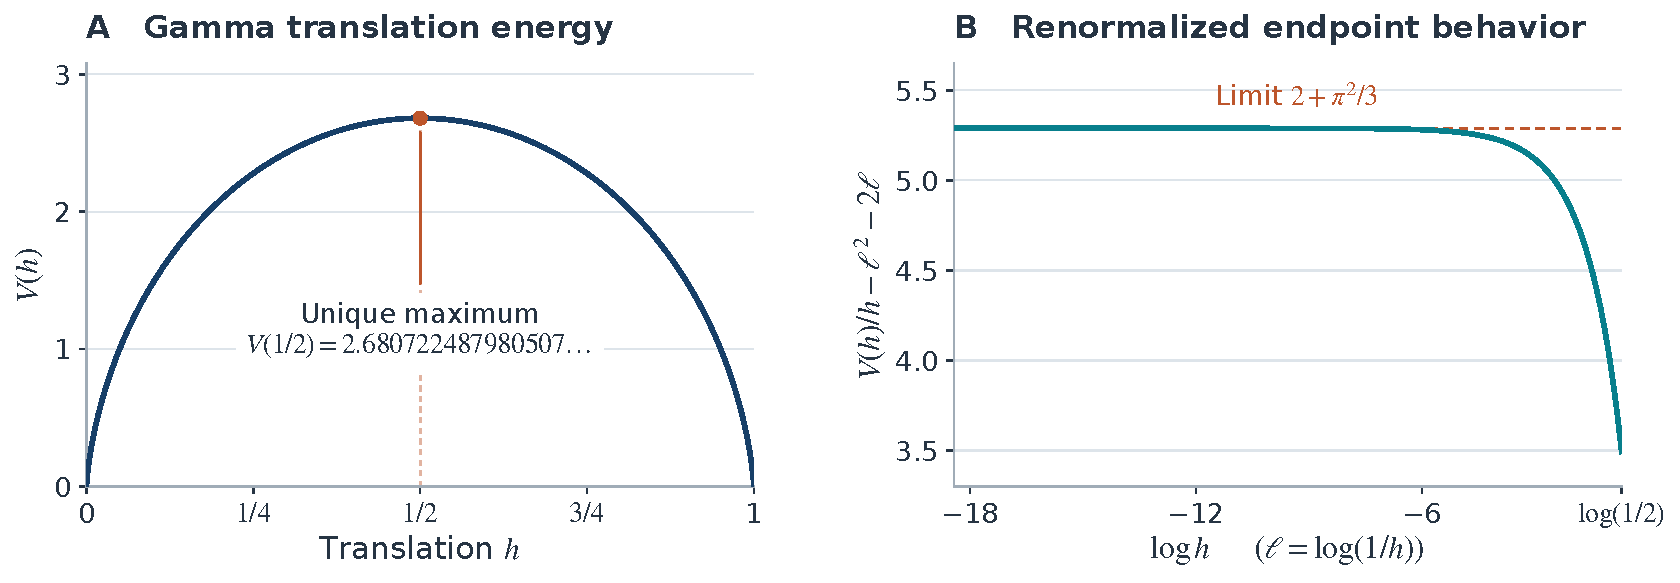
\includegraphics[width=\textwidth]{figures/gamma_translation.pdf}
\caption{The Gamma translation energy and its renormalized endpoint
limit. The left panel illustrates the proved strict concavity and
half-period maximum. The right subtracts the explicit logarithmic
terms, leaving a limit of $2+\pi^2/3$. Curves are evaluated from
the convergent series with its analytic truncation bound.}
\label{fig:gamma-energy}
\end{figure}

\begin{proof}
Twice differentiating \eqref{eq:gamma-hurwitz}, using the Laurent
expansion at $1$ before evaluating removable singularities, gives
\begin{equation}\label{eq:Vsecond}
 V''(h)=2\left(\gamma_1(h)+\gamma_1(1-h)-\frac{\pi^2}{3}\right).
\end{equation}
We prove a sufficient strict bound entirely analytically. The derivative
tower gives, by an absolutely convergent series,
\[
 \gamma_1'(a)=\sum_{m=0}^{\infty}
                 \frac{1-\log(m+a)}{(m+a)^2}.
\]
For $0<a\leq1$, its $m=0$ term is at least $1$, its $m=1$ term is
positive, and the possibly negative remaining terms have total magnitude
at most $\sum_{m\geq2}\log m/m^2$. The function $\log x/x^2$
is decreasing for $x\geq2$, so
\[
 -\zeta'(2)
 \leq\frac{\log2}{4}+\frac{\log3}{9}
         +\int_3^\infty\frac{\log x}{x^2}\,dx
 =\frac{\log2}{4}+\frac{4\log3}{9}+\frac13
 <\frac{359}{360}<1.
\]
The strict rational bound uses $\log2<7/10$ and $\log3<11/10$.
Hence $\gamma_1'(a)>0$ on $(0,1]$.

The sum-integral definition of $\gamma_1$, and decrease of
$\log x/x$ for $x\geq3$, also give
\[
 \gamma_1(1)
 \leq\frac{\log2}{2}+\frac{\log3}{3}
                         -\frac{\log^23}{2}
 <\frac{43}{60}<1<\frac{\pi^2}{6}.
\]
Thus both Stieltjes constants in \eqref{eq:Vsecond} are less than
$\pi^2/6$, proving strict concavity. Periodic translation invariance
gives $V(1-h)=V(h)$, so the unique maximum is at $1/2$.
Finally insert $\zeta(s,1/2)=(2^s-1)\zeta(s)$ and its first two
order derivatives into \eqref{eq:gamma-hurwitz}. This gives
\eqref{eq:Vmax}. The displayed decimal is a diagnostic evaluation;
neither the sign proof nor optimality depends on it.
\end{proof}

\subsection{Explicit derivatives, polygamma forms, and a definite primitive}

The exact Gamma energy also has useful identities beyond its second
derivative. For every integer $m\geq1$ and $0<h<1$,
\begin{equation}\label{eq:V-higher}
 V^{(m+2)}(h)=2\bigl[\gamma_1^{(m)}(h)
                         +(-1)^m\gamma_1^{(m)}(1-h)\bigr].
\end{equation}
The classical derivative tower takes the particularly simple form
\begin{equation}\label{eq:gamma1-polygamma}
 \gamma_1^{(m)}(a)=(-1)^{m+1}m!\zeta'(m+1,a)
                         +H_m\psi^{(m)}(a),\qquad a>0.
\end{equation}
Indeed, compare the coefficient of $u$ in
\[
 \partial_a^m\zeta(1+u,a)
 =(-1)^m(1+u)_m\zeta(m+1+u,a),
\]
using $\partial_u(1+u)_m|_{u=0}=m!H_m$ and
$\psi^{(m)}(a)=(-1)^{m+1}m!\zeta(m+1,a)$.
Equations \eqref{eq:V-higher}--\eqref{eq:gamma1-polygamma}
therefore express all higher shift derivatives directly in polygamma
functions and Hurwitz order derivatives at positive integers. The
identities apply on the open interval; the endpoint derivatives
generally diverge.

For the primitive, define
\[
 W_j(h)=\zeta^{(j)}(-2,h)-\zeta^{(j)}(-2,1-h),\qquad
 a_0=2+\frac{\pi^2}{3}.
\]
Corollary~\ref{cor:shift-primitive}, with $m=1$ followed by
$\partial_s\partial_t$ at zero, gives
\begin{align}
 \int_0^h V(v)\,dv={}&\frac{W_2(h)}2+\frac{3W_1(h)}2
            +\left(\frac74+\frac{\pi^2}{6}\right)W_0(h)\notag\\
 &-2h\bigl[\zeta''(-1)+2\zeta'(-1)+a_0\zeta(-1)\bigr].
 \label{eq:V-primitive}
\end{align}
There is no omitted integration constant: all $W_j$ vanish at zero
by continuous extension, since $h^2\log^j h\to0$. At $h=1$ this
becomes the exact mean-energy identity
\begin{equation}\label{eq:V-mean}
 \int_0^1 V(h)\,dh
 =-2\zeta''(-1)-4\zeta'(-1)+\frac13+\frac{\pi^2}{18}.
\end{equation}
It is also twice the centered second moment of $\log\Gamma$ on
$(0,1)$, as follows directly by averaging the defining translation.

\subsection{A convergent identity for the first Stieltjes constant}

The coefficients removed in \eqref{eq:gamma-series} are all positive.
Indeed, for $p\geq3$,
\[
 H_{p-1}\zeta(p)+\zeta'(p)
 \geq\frac32-\sum_{k\geq2}\frac{\log k}{k^3}
 \geq\frac32-\frac{\log2}{4}-\frac1{16}>0.
\]
They are $O(\log j/j^2)$ after the displayed prefactor in
\eqref{eq:gamma-series}. The series consequently extends uniformly to
$0\leq h\leq1$. Letting $h\uparrow1$ and using $V(1)=0$ proves
\begin{equation}\label{eq:gamma1-odd}
 \boxed{\quad
 \gamma_1=-1+\sum_{j=2}^{\infty}
   \frac{\zeta'(2j-1)+H_{2j-2}\zeta(2j-1)}{j(2j-1)}.
 \quad}
\end{equation}
This form is slow but has positive summands. Subtracting the elementary
harmonic contribution makes it geometrically convergent.

\begin{corollary}[An accelerated odd-zeta identity]\label{cor:gamma1-fast}
One has
\begin{equation}\label{eq:gamma1-fast}
 \boxed{\quad
 \gamma_1=2\log2-\log^22-1+
 \sum_{j=2}^{\infty}
 \frac{\zeta'(2j-1)+H_{2j-2}(\zeta(2j-1)-1)}{j(2j-1)}.
 \quad}
\end{equation}
If the sum is truncated at $j=J\geq2$, the absolute tail is bounded by
\begin{equation}\label{eq:gamma1-tail}
 \frac{16}{3}\,
 \frac{2+\log(2J+2)}{(J+1)^2}\,4^{-(J+1)}.
\end{equation}
\end{corollary}

\begin{proof}
The even part of $\sum_{n\geq0}H_nx^n=-\log(1-x)/(1-x)$ gives
\begin{align*}
 \sum_{j=2}^{\infty}\frac{H_{2j-2}}{j(2j-1)}
 &=2\int_0^1(1-x)\sum_{m\geq1}H_{2m}x^{2m}\,dx\\
 &=-\int_0^1\log(1-x)\,dx
     -\int_0^1\frac{1-x}{1+x}\log(1+x)\,dx\\
 &=2\log2-\log^22.
\end{align*}
Tonelli or absolute convergence justifies the interchange. Subtract
this value from \eqref{eq:gamma1-odd}.

For $p\geq3$, integral comparison yields
\[
 \zeta(p)-1\leq2^{1-p},\qquad
 |\zeta'(p)|\leq2\cdot2^{-p}.
\]
Together with $H_{2j-2}\leq1+\log(2j-2)$, each absolute summand
in the accelerated series is at most
$4(2+\log(2j))4^{-j}/j^2$. The factor
$(2+\log(2j))/j^2$ decreases, and summing the geometric tail gives
\eqref{eq:gamma1-tail}.
\end{proof}

For actual evaluation this tail bound is combined with controlled
evaluation of the finitely many zeta values and derivatives. A small
formal tail alone does not certify floating-point special-function
evaluations. The accompanying program explicitly labels its numerical
comparisons as diagnostics.

The same positivity gives useful global estimates. If
$A(h)=h(\log^2h-2\log h+2+\pi^2/3)
 +(2\gamma_1-\pi^2/3)h^2$, then
\begin{equation}\label{eq:V-bounds}
 A(h)-2(1+\gamma_1)h^4
 \leq V(h)\leq
 A(h)-\frac{\zeta'(3)+\tfrac32\zeta(3)}{3}h^4,
 \qquad 0<h<1.
\end{equation}
The left inequality is sharp at $h=1$ by continuity, and the right
has the exact first omitted coefficient at zero. For computation one
may replace $h$ by $\min(h,1-h)$ before using the convergent series.

% END article/02_gamma.tex


% BEGIN article/03_euler_transition.tex
\section{A uniform transition at outer order one}
\label{eutrans:sec:main}

This section proves the near-critical reversal conjecture
\texttt{research:conj:crossing} in the pinned continuation
\texttt{tetralogarithm-euler-polynomial-zeros} and determines its first
logarithmic correction. The distinction between an expansion for fixed
parameters and an expansion uniform at an integer outer order is essential:
the coefficient of the algebraic density vanishes at outer order one,
while an exponentially small density survives. Both contributions are
of the same size at the reversal.

\subsection{Definitions and the inherited sign theorem}

For $a,b>0$, write
\[
 F_{a,b}(z)=\sum_{n\geq1}\frac{H_{n-1}^{(b)}}{n^a}z^n,
 \qquad H_m^{(b)}=\sum_{j=1}^m j^{-b},
 \qquad g_{a,b}=\operatorname{Im}F_{a,b}(i),
\]
where the boundary value is its analytic continuation. Define
\[
 f_n=\frac{H_{2n}^{(b)}}{(2n+1)^a},\qquad
 d_j=\sum_{n=0}^j(-1)^n\binom jn f_n,\qquad
 E_N=\sum_{j=0}^{N-1}\frac{d_j}{2^{j+1}},\qquad
 R_N(a,b)=2^N(E_N-g_{a,b}).
\]
The axis $a=0$ uses the same analytic convention. The comparison of
interest fixes the total order:
\[
 \mathcal D_{a,b}(N)=R_N(a,b)-R_N(0,a+b).
\]
Set
\begin{align}
 h_b(T)&=\frac1{\Gamma(b)}\int_T^\infty
                    \frac{v^{b-1}}{e^v-1}\,dv,
 & I^ah_b(T)&=\frac1{\Gamma(a)}\int_0^T(T-v)^{a-1}h_b(v)\,dv,
 \label{eutrans:eq:seed}\\
 D_{a,b}(T)&=(I^ah_b)'(T)
              +\frac{T^{a+b-1}}{\Gamma(a+b)(e^T-1)},
 & q(T)&=1-e^{-2T}.
 \label{eutrans:eq:density}
\end{align}
The exact compensated Euler formula yields
\begin{equation}\label{eutrans:eq:interpolation}
 \mathcal D_{a,b}(s)=-\int_0^\infty D_{a,b}(T)
          \frac{e^{-T}q(T)^s}{1+e^{-2T}}\,dT,
 \qquad s\geq1.
\end{equation}
It agrees with the preceding definition at integers and supplies the
real interpolation used below. All its derivatives in $s$ are ordinary
absolutely convergent integrals. In fact, with
$\ell(T)=-\log q(T)>0$,
\begin{equation}\label{eutrans:eq:derivatives}
 (-1)^r\mathcal D_{a,b}^{(r)}(s)
 =-\int_0^\infty D_{a,b}(T)
    \frac{e^{-T}q(T)^s\ell(T)^r}{1+e^{-2T}}\,dT.
\end{equation}

The prior phase theorem \cite{RepoEuler} establishes the following facts. For $0<a<1$,
$D_{a,b}(T)$ has precisely one sign change, from positive to negative.
For every integer $r\geq0$, $\mathcal D_{a,b}^{(r)}$ has one simple
zero $\nu_r(a,b)>1$, and
\[
 1<\nu_0(a,b)<\nu_1(a,b)<\cdots.
\]
The sign of $(-1)^r\mathcal D_{a,b}^{(r)}$ is negative before that
zero and positive afterwards. In particular $\nu_0=\nu$ is the
reversal index, while $\nu_1$ is the location of the unique positive
maximum of $\mathcal D_{a,b}$. These facts can also be checked directly from
\eqref{eutrans:eq:derivatives}: the ratio of the weights at two $s$
values is strictly increasing in $T$, so subtracting its value at the
density crossing proves the one-zero property. A similar comparison
with the strictly decreasing function $\ell(T)$ orders the derivative
zeros. We use this already proved sign theorem to identify the unique
roots isolated by our uniform estimates.

Throughout the uniform statements, $B=[b_-,b_+]$ is any fixed compact
interval in $(0,\infty)$ and $r$ is a fixed nonnegative integer. Put
\[
 a=1-\varepsilon,\qquad
 \lambda=\log(1/\varepsilon),\qquad p=b+1.
\]
Choose $\varepsilon_0<\min(1/2,b_-/2)$. In particular, the parameters
used here are strictly in the finite-measure region $a+b>1$; no
unweighted hypersingular integral is introduced in this joint limit.

\subsection{The reversal asymptotic and its correction}

Define
\begin{align}
 K_{b,r}&=b\Gamma(b+1)\zeta(b+1)
              \frac{\Gamma(r+1/2)}{\Gamma(r+1)},
 \label{eutrans:eq:K}\\
 \delta_{b,r}&=b-\frac b2\psi(r+1)-\frac12\psi(r+1/2)
      -\frac{(b+1)\zeta(b+2)}{2\zeta(b+1)}.
 \label{eutrans:eq:delta}
\end{align}
All zeta values in these constants lie in their absolutely convergent
range, and both gamma factors have positive arguments.

\begin{theorem}[Near-critical reversal and derivative zeros]
\label{eutrans:thm:crossing}
As $\varepsilon\downarrow0$, uniformly for $b\in B$ and each fixed $r$,
\begin{align}
 \frac12\log\nu_r(1-\varepsilon,b)
 ={}&\lambda+p\log\lambda-\log K_{b,r}\notag\\
 &+\frac{p^2\log\lambda-p\log K_{b,r}+\delta_{b,r}}{\lambda}
 +O_{B,r}\left(\frac{(\log\lambda)^2}{\lambda^2}\right).
 \label{eutrans:eq:Lroot}
\end{align}
Equivalently,
\begin{align}
 \nu_r(1-\varepsilon,b)
 ={}&\frac{\lambda^{2b+2}}{K_{b,r}^2\varepsilon^2}
 \Biggl[1+
 \frac{2p^2\log\lambda-2p\log K_{b,r}+2\delta_{b,r}}{\lambda}
 \notag\\
 &\hspace{30mm}+O_{B,r}\left(\frac{(\log\lambda)^2}{\lambda^2}\right)
 \Biggr].
 \label{eutrans:eq:nuroot}
\end{align}
For $r=0$, this proves the proposed leading law
\begin{equation}\label{eutrans:eq:conjecture}
 \nu(1-\varepsilon,b)\sim
 \frac{(\log(1/\varepsilon))^{2b+2}}
 {\pi b^2\Gamma(b+1)^2\zeta(b+1)^2\varepsilon^2}.
\end{equation}
Its first correction uses
\begin{equation}\label{eutrans:eq:delta0}
 \delta_{b,0}=b+\frac{b+1}{2}\gamma+\log2
                   -\frac{(b+1)\zeta(b+2)}{2\zeta(b+1)}.
\end{equation}
\end{theorem}

The $\log\log(1/\varepsilon)/\log(1/\varepsilon)$ correction is
substantial at accessible parameter values. Keeping the implicit
logarithmic equation gives a more useful approximation.

\begin{corollary}[An approximation in terms of Lambert $W$]
\label{eutrans:cor:lambert}
For sufficiently small $\varepsilon$, put
\begin{equation}\label{eutrans:eq:Lambert}
 \widehat L_{b,r}=-p\,W_{-1}\left(
             -\frac{(K_{b,r}\varepsilon)^{1/p}}p\right).
\end{equation}
Here $W_{-1}$ is the real branch with values at most $-1$.
Then $\widehat L_{b,r}>p$ and, uniformly for $b\in B$,
\begin{equation}\label{eutrans:eq:Lambert-correction}
 \frac12\log\nu_r(1-\varepsilon,b)
 =\widehat L_{b,r}+
       \frac{\delta_{b,r}}{\widehat L_{b,r}-p}
       +O_{B,r}(\widehat L_{b,r}^{-2}).
\end{equation}
\end{corollary}

We now prove the theorem with the estimates that control both limits.

\subsection{Preserving the vanishing algebraic amplitude}

The seed moments are
\begin{equation}\label{eutrans:eq:moments}
 m_j(b)=\int_0^\infty v^j h_b(v)\,dv
       =\frac{(b)_{j+1}}{j+1}\zeta(b+j+1).
\end{equation}
Indeed, Tonelli first integrates $v^j$ up to the outer variable, and
then expansion of $(e^v-1)^{-1}$ gives a sum of gamma integrals. In
particular,
\[
 m_0=b\zeta(b+1),\qquad
 m_1=\frac{b(b+1)}2\zeta(b+2).
\]
Every fixed moment is uniformly bounded as $b$ ranges over $B$.

\begin{lemma}[A uniform density estimate with an $\varepsilon$ factor]
\label{eutrans:lem:density}
For some $M$ depending only on $B$, uniformly for $T\geq2$,
$b\in B$, and $0\leq\varepsilon\leq\varepsilon_0$,
\begin{align}
 (I^{1-\varepsilon}h_b)'(T)
 ={}&h_b(T)-\frac{\varepsilon T^{-1-\varepsilon}}
                  {\Gamma(1-\varepsilon)}
       \left[m_0+\frac{(1+\varepsilon)m_1}{T}
                    +O_B(T^{-2})\right]\notag\\
 &+O_B\left(\varepsilon e^{-T/2}(1+T)^M\right).
 \label{eutrans:eq:uniform-density}
\end{align}
Moreover,
\begin{equation}\label{eutrans:eq:h-infty}
 h_b(T)=\frac{e^{-T}T^{b-1}}{\Gamma(b)}
                   \{1+O_B(T^{-1})\}.
\end{equation}
The $O_B(T^{-2})$ term in \eqref{eutrans:eq:uniform-density} is
inside the bracket multiplied by $\varepsilon$.
\end{lemma}

\begin{proof}
For $T>0$, the regularized differentiation formula is
\begin{equation}\label{eutrans:eq:Marchaud}
 (I^{1-\varepsilon}h_b)'(T)
 =\frac1{\Gamma(1-\varepsilon)}\left[
 T^{-\varepsilon}h_b(T)
 +\varepsilon\int_0^T
       \frac{h_b(T)-h_b(v)}{(T-v)^{1+\varepsilon}}\,dv\right].
\end{equation}
The integral is absolutely convergent. At $v=0$, $h_b(v)$ is
locally integrable; at $v=T$, the numerator is $O(T-v)$ and
$\varepsilon<1$. One way to derive the identity without using an
endpoint value $h_b(0)$ is to replace the fractional kernel by
$(T-v+\eta)^{-\varepsilon}$, differentiate, subtract $h_b(T)$ in
the differentiated integral, and let $\eta\downarrow0$. Dominated
convergence applies to the subtracted integral and to the original
fractional integral on compact positive $T$ intervals. Its boundary
term tends to $T^{-\varepsilon}h_b(T)$. The same computation at
$\varepsilon=0$ gives $(I^1h_b)'=h_b$.

Split the integral in \eqref{eutrans:eq:Marchaud} at $v=T/2$.
On the first part retain $-h_b(v)$ and expand
\[
 (T-v)^{-1-\varepsilon}=T^{-1-\varepsilon}
 \left[1+(1+\varepsilon)\frac vT
                  +O\left(\frac{v^2}{T^2}\right)\right].
\]
The Taylor bound is uniform for $0\leq v/T\leq1/2$ and the chosen
compact $\varepsilon$ interval. Replacing the truncated moments by
the full moments changes the result by an exponential error, since
$h_b(v)$ decays exponentially at infinity with a uniform polynomial
bound. The second moment bounds the Taylor remainder and yields
the bracket in \eqref{eutrans:eq:uniform-density}.

Here are bounds for the remaining terms. For $u\geq1$,
\[
 |h_b(u)|+|h_b'(u)|
       \leq C_B e^{-u}(1+u)^{M_0}.
\]
For $v\geq T/2$, the mean value theorem gives
\[
 |h_b(T)-h_b(v)|
 \leq C_B e^{-T/2}(1+T)^{M_0}\min(T-v,1).
\]
Consequently its integral against $(T-v)^{-1-\varepsilon}$ is at
most $C_Be^{-T/2}(1+T)^{M_0+1}$, uniformly in $\varepsilon$:
the integral on $0<T-v<1$ is bounded by $(1-\varepsilon_0)^{-1}$,
and the rest by $1+\log T$.
The $h_b(T)$ contribution on $v<T/2$ satisfies the same type of
bound. Finally
\[
 \left|\frac{T^{-\varepsilon}}{\Gamma(1-\varepsilon)}-1\right|
                \leq C\varepsilon(1+\log T),
\]
by the mean value theorem in $\varepsilon$. Multiplication by
$h_b(T)$ absorbs this discrepancy in the exponential error. Every
discarded term in this paragraph carries the prefactor
$\varepsilon$ from \eqref{eutrans:eq:Marchaud}, or the same factor
from the last inequality. Increasing $M$ proves
\eqref{eutrans:eq:uniform-density}.

For \eqref{eutrans:eq:h-infty}, expand the Bose denominator as
$e^{-v}\{1+O(e^{-v})\}$. In the leading integral set $v=T+u$,
factor $e^{-T}T^{b-1}$, and use
$(1+u/T)^{b-1}=1+O_B(u(1+u)^{M_1}/T)$ inside its exponential
integral. This proves the estimate uniformly on $B$.
\end{proof}

\subsection{A joint expansion under the Euler kernel}

Put
\begin{align}
 A_{b,r}&=\frac{m_0(b)\Gamma(r+1/2)}2,
 & B_{b,r}&=\frac{\Gamma(r+1)}{2\Gamma(b+1)},
 \label{eutrans:eq:AB}\\
 \alpha_{b,r}&=\frac12\psi(r+1/2)+\frac{m_1(b)}{m_0(b)},
 & \beta_{b,r}&=b-\frac b2\psi(r+1).
 \label{eutrans:eq:alphabeta}
\end{align}
Thus $K_{b,r}=A_{b,r}/B_{b,r}$ and
$\delta_{b,r}=\beta_{b,r}-\alpha_{b,r}$.

\begin{lemma}[Uniform competition of two scales]
\label{eutrans:lem:joint}
Let $L=\tfrac12\log s$ and $\lambda=\log(1/\varepsilon)$. Uniformly
for $b\in B$ and $\lambda/2\leq L\leq2\lambda$, as
$\varepsilon\downarrow0$,
\begin{align}
 (-1)^r\mathcal D_{1-\varepsilon,b}^{(r)}(s)
 ={}&\varepsilon A_{b,r}s^{-r-1/2}L^{-1}
       \{1+\alpha_{b,r}/L+O_{B,r}(L^{-2})\}\notag\\
 &-B_{b,r}s^{-r-1}L^b
       \{1+\beta_{b,r}/L+O_{B,r}(L^{-2})\}.
 \label{eutrans:eq:joint}
\end{align}
The two remainder terms are bounded separately by their respective
displayed scales. In particular the estimate remains useful where
the leading terms cancel.
\end{lemma}

\begin{proof}
Insert Lemma~\ref{eutrans:lem:density} into
\eqref{eutrans:eq:density} and \eqref{eutrans:eq:derivatives}. The
change of variable $t=\sqrt{s}e^{-T}$ gives $T=L-\log t$ and
$e^{-T}\,dT=-s^{-1/2}\,dt$. On the central interval
$s^{-1/4}\leq t\leq s^{1/4}$ one has $T\in[L/2,3L/2]$ and
\begin{align*}
 \frac{(1-t^2/s)^s}{1+t^2/s}&\longrightarrow e^{-t^2},\\
 \{s[-\log(1-t^2/s)]\}^r&\longrightarrow t^{2r}.
\end{align*}
Their differences from the limits have integrals bounded by
$O_r(s^{-1})$ times fixed Gaussian moments. For example, when
$t^2/s\leq1/2$,
\[
 \left|\frac{(1-t^2/s)^s}{1+t^2/s}-e^{-t^2}\right|
 \leq C s^{-1}e^{-t^2}(t^2+t^4),
\]
and the second replacement has an analogous bound with a further
fixed polynomial in $t$. The powers of $T$ remain comparable to
their powers of $L$ on this central interval.

The tails require no uniformity assumption beyond the stated window.
For $T<L/2$, use $q(T)^s\leq\exp(-s e^{-2T})\leq\exp(-e^L)$.
The local bounds can be made explicit: for $0<T\leq1$,
\[
 |D_{1-\varepsilon,b}(T)|\leq C_B
 \bigl(T^{-\varepsilon_0}+T^{b_--1-\varepsilon_0}\bigr)
                                  (1+|\log T|).
\]
Indeed $h_b(T)\leq C_B(1+T^{b_--1})(1+|\log T|)$ follows by
splitting its integral at one; insertion in the compensated
derivative formula, or its beta-integral form
\eqref{eutrans:eq:numerical-density}, gives the displayed estimate.
Since $\varepsilon_0<b_-/2$ and $\varepsilon_0<1/2$, it is
integrable even after multiplication by the additional fixed powers
of $\log T$ coming from $\ell(T)^r$. For $T\geq1$ the density lemma
gives a common polynomial bound. This entire contribution is smaller
than either displayed scale times every power of $L^{-1}$; the
window implies $e^{-2L}\leq\varepsilon\leq e^{-L/2}$.
For $T>3L/2$, equivalently $0<t<s^{-1/4}$, each algebraic contribution
retains its factor $\varepsilon$ and is bounded by the elementary
moments of $t^{2r}$ over this shrinking interval. Exponential
contributions have the extra factor $t$ and are bounded still more
strongly. Logarithmic factors are harmless, since all fixed moments
of $t^c|\log t|^j$ at zero are finite for $c>-1$.

For clarity, the exponential error in
\eqref{eutrans:eq:uniform-density} contributes at most
\[
 O_{B,r}\left(\varepsilon s^{-r-3/4}(1+L)^M\right).
\]
Its ratio to the algebraic scale is
$O_{B,r}(s^{-1/4}(1+L)^{M+1})$, which is smaller than $L^{-2}$
uniformly in the window. The $O(e^{-2T})$ terms produced by the
Bose denominator are likewise negligible relative to the appropriate
exponential scale. These estimates explain why simply deleting an
exponential density in the fixed-parameter expansion would be invalid.

It remains to compute the first corrections. Uniformly in the window,
$\varepsilon\log L=o(L^{-k})$ for every fixed $k$.
Thus $L^{-\varepsilon}$, $\Gamma(1-\varepsilon)^{-1}$, and
$\Gamma(b+1-\varepsilon)^{-1}$ may be replaced by their values at
$\varepsilon=0$ at the required relative accuracy. For any exponent
$c$ in a fixed compact real set, Taylor's theorem on
$|\log t|\leq L/2$ gives
\[
 (L-\log t)^c=L^c\left[
         1-\frac{c\log t}{L}
          +O\left(\frac{(\log t)^2}{L^2}\right)\right].
\]
The full moments needed after extending the central interval are
\begin{align*}
 \int_0^\infty t^{2r}e^{-t^2}\,dt&=\frac12\Gamma(r+1/2),
 &\frac{\int_0^\infty t^{2r}e^{-t^2}\log t\,dt}
       {\int_0^\infty t^{2r}e^{-t^2}\,dt}
       &=\frac12\psi(r+1/2),\\
 \int_0^\infty t^{2r+1}e^{-t^2}\,dt&=\frac12\Gamma(r+1),
 &\frac{\int_0^\infty t^{2r+1}e^{-t^2}\log t\,dt}
       {\int_0^\infty t^{2r+1}e^{-t^2}\,dt}
       &=\frac12\psi(r+1).
\end{align*}
The algebraic density consequently gives $A_{b,r}$ and
$\alpha_{b,r}$. The dominant positive density
$e^{-T}T^b/\Gamma(b+1)$ gives the correction
$-b\psi(r+1)/2$; the retained seed $h_b(T)$ gives the additional
$b/L$, because $\Gamma(b+1)/\Gamma(b)=b$. Hence its coefficient is
$\beta_{b,r}$. The separately bounded second logarithmic moments
prove both remainders in \eqref{eutrans:eq:joint}.
\end{proof}

\subsection{Locating and expanding the unique zero}

\begin{proof}[Proof of Theorem~\ref{eutrans:thm:crossing}]
Define
\[
 S_{\varepsilon,b,r}=
        \frac{\lambda^{2p}}{K_{b,r}^2\varepsilon^2}.
\]
For $s=xS_{\varepsilon,b,r}$ and $x$ in any fixed compact interval
of $(0,\infty)$, $L=\lambda+p\log\lambda-\log K_{b,r}
+\tfrac12\log x$, so $L/\lambda\to1$ uniformly for $b\in B$.
In \eqref{eutrans:eq:joint}, the ratio of the first positive scale
to the second positive scale is
\[
 \varepsilon K_{b,r}\sqrt{s}\,L^{-p}
                =\sqrt{x}(\lambda/L)^p\longrightarrow\sqrt{x}.
\]
Thus the comparison has opposite signs at any fixed $x<1$ and
fixed $x>1$, uniformly for $b\in B$. The inherited uniqueness
theorem identifies its zero and proves
\[
 \nu_r(1-\varepsilon,b)/S_{\varepsilon,b,r}\longrightarrow1.
\]
This first localization justifies using the same window at the zero;
the window has not been assumed as an unproved property of $\nu_r$.

At the zero set $L_r=\tfrac12\log\nu_r$. Equating the two terms
of \eqref{eutrans:eq:joint} and dividing their positive factors gives
\[
 \varepsilon K_{b,r}e^{L_r}L_r^{-p}
       =1+\frac{\delta_{b,r}}{L_r}+O_{B,r}(L_r^{-2}).
\]
Taking logarithms yields the uniform equation
\begin{equation}\label{eutrans:eq:root-equation}
 L_r=\lambda+p\log L_r-\log K_{b,r}
                +\frac{\delta_{b,r}}{L_r}+O_{B,r}(L_r^{-2}).
\end{equation}
First $L_r=\lambda+O_B(\log\lambda)$, and substitution once more
gives $L_r=\lambda+p\log\lambda-\log K_{b,r}
+O_{B,r}(\log\lambda/\lambda)$. Expand $\log L_r$ about
$\lambda$ in \eqref{eutrans:eq:root-equation}. The result is
\eqref{eutrans:eq:Lroot}; Taylor's remainder is
$O_{B,r}((\log\lambda)^2/\lambda^2)$. Exponentiating gives
\eqref{eutrans:eq:nuroot}. The cases $r=0$ follow from
$\Gamma(1/2)=\sqrt\pi$, $\psi(1)=-\gamma$, and
$\psi(1/2)=-\gamma-2\log2$.
\end{proof}

\begin{proof}[Proof of Corollary~\ref{eutrans:cor:lambert}]
The number $\widehat L=\widehat L_{b,r}$ in
\eqref{eutrans:eq:Lambert} is the large solution of
\[
 \widehat L-p\log\widehat L=\lambda-\log K_{b,r}.
\]
It satisfies $\widehat L\sim\lambda$, uniformly on $B$.
On that range the derivative of $L-p\log L$ is
$1-p/L$, bounded away from zero. Comparing with
\eqref{eutrans:eq:root-equation} first gives
$L_r-\widehat L=O_{B,r}(\widehat L^{-1})$. One Taylor expansion
then gives
\[
 (1-p/\widehat L)(L_r-\widehat L)
     =\delta_{b,r}/\widehat L+O_{B,r}(\widehat L^{-2}),
\]
which proves \eqref{eutrans:eq:Lambert-correction}.
\end{proof}

\subsection{A universal profile and the positive maximum}

For $r=0$, abbreviate $K_b=K_{b,0}$ and set
\begin{equation}\label{eutrans:eq:profile-scales}
 S_{\varepsilon,b}=\frac{\lambda^{2b+2}}{K_b^2\varepsilon^2},
 \qquad
 M_{\varepsilon,b}=\frac{\pi b^2\Gamma(b+1)\zeta(b+1)^2}{2}
                  \frac{\varepsilon^2}{\lambda^{b+2}}.
\end{equation}

\begin{theorem}[Universal profile and derivative-root ratios]
\label{eutrans:thm:profile}
For every compact $X\subset(0,\infty)$ and every fixed nonnegative
integer $m$,
\begin{equation}\label{eutrans:eq:profile}
 \frac{\mathcal D_{1-\varepsilon,b}(S_{\varepsilon,b}x)}
             {M_{\varepsilon,b}}
       \longrightarrow x^{-1/2}-x^{-1}
       \qquad\hbox{in }C^m(X),
\end{equation}
uniformly for $b\in B$. Consequently, for every fixed $r$,
\begin{equation}\label{eutrans:eq:root-ratios}
 \frac{\nu_r(1-\varepsilon,b)}{\nu_0(1-\varepsilon,b)}
       \longrightarrow
       \left\{\frac{\sqrt\pi\Gamma(r+1)}{\Gamma(r+1/2)}\right\}^2
       =\left\{\frac{4^r}{\binom{2r}{r}}\right\}^2.
\end{equation}
In particular the maximum is attained at an index asymptotic to
$4\nu_0$, and its height satisfies
\begin{equation}\label{eutrans:eq:height}
 \max_{s\geq1}\mathcal D_{1-\varepsilon,b}(s)
 \sim \frac{\pi b^2\Gamma(b+1)\zeta(b+1)^2}{8}
                  \frac{\varepsilon^2}{\lambda^{b+2}}.
\end{equation}
The same height asymptotic holds when the maximum is restricted to
integer truncation orders. Any maximizing integer is one of the two
integers adjacent to $\nu_1$. The first integer with a strictly
positive comparison is $\lfloor\nu_0\rfloor+1$ and therefore has
the same asymptotic as \eqref{eutrans:eq:conjecture}.
\end{theorem}

\begin{figure}[tbp]
\centering
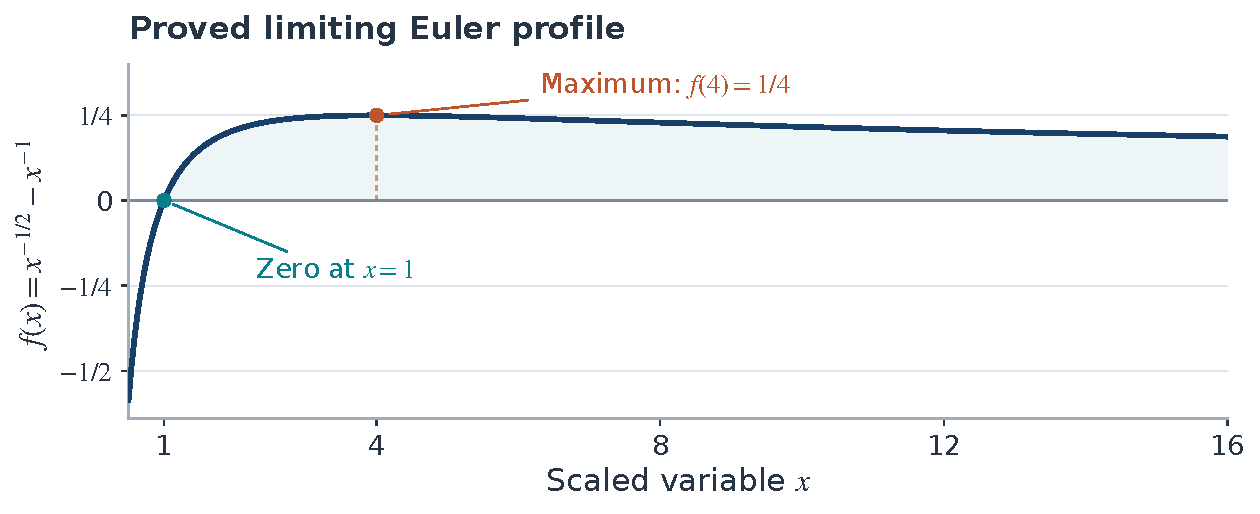
\includegraphics[width=0.90\textwidth]{figures/euler_limiting_profile.pdf}
\caption{The proved limiting profile $x^{-1/2}-x^{-1}$ from
Theorem~\ref{eutrans:thm:profile}, shown for $1/2\leq x\leq16$.
Its zero at one locates the reversal scale and its maximum at four
locates the later positive maximum. This is the limiting function,
not a finite-$\varepsilon$ numerical comparison.}
\label{fig:euler-profile}
\end{figure}

\begin{proof}
The two scales in \eqref{eutrans:eq:joint}, evaluated at
$s=S_{\varepsilon,b}x$, both equal $M_{\varepsilon,b}$ at $x=1$
to leading order. Their $x$ powers are $x^{-1/2}$ and $x^{-1}$.
For every $r\leq m$, the already justified differentiated integral
in Lemma~\ref{eutrans:lem:joint} gives
\[
 \frac{S_{\varepsilon,b}^r
             \mathcal D_{1-\varepsilon,b}^{(r)}
                        (S_{\varepsilon,b}x)}{M_{\varepsilon,b}}
 \longrightarrow(-1)^r\left[
     (1/2)_r x^{-r-1/2}-r!x^{-r-1}\right]
\]
uniformly on $X$. This proves $C^m$ convergence directly, rather than
by differentiating an undifferentiated asymptotic. The root ratios
follow either from these limiting derivatives and uniqueness or
from \eqref{eutrans:eq:nuroot}. The gamma duplication formula gives
the central-binomial expression.

The limiting profile has its unique positive maximum at $x=4$, with
value $1/4$. The inherited global one-maximum theorem places the
actual maximum at $\nu_1$, and \eqref{eutrans:eq:root-ratios} puts
$\nu_1/S_{\varepsilon,b}\to4$. Evaluation of the uniform profile
there gives \eqref{eutrans:eq:height}. No global maximum is inferred
solely from convergence on compact $x$ intervals.
Strict increase before $\nu_1$ and strict decrease afterwards reduce
the integer maximum to the adjacent integers; their rescaled
locations tend to four as well. The asserted first positive integer
follows from the strict sign classification at $\nu_0$.
\end{proof}

\subsection{Verification, integration status, and further questions}

The numerical verifier evaluates the exact density through the
cancellation-free identity
\begin{align}\label{eutrans:eq:numerical-density}
 D_{1-\varepsilon,b}(T)
 ={}&\frac{T^{-\varepsilon}}{\Gamma(1-\varepsilon)}
  \left[h_b(T)-\frac1{\Gamma(b)}\int_0^T
   \frac{v^{b-1}\bigl\{(1-v/T)^{-\varepsilon}-1\bigr\}}
        {e^v-1}\,dv\right]\notag\\
 &+\frac{T^{b-\varepsilon}}{\Gamma(b+1-\varepsilon)(e^T-1)}.
\end{align}
It uses \texttt{expm1} and \texttt{log1p} for the small numerator.
This expression follows by interchanging integrals in $I^ah_b$
before differentiation and is independent of the truncated large-$T$
expansion used in the proof. At $b=1$ it uses
$h_1(T)=-\log(1-e^{-T})$; at $b=2$ it uses
$h_2(T)=\operatorname{Li}_2(e^{-T})-T\log(1-e^{-T})$.
The outer integral is evaluated after the exact Gaussian change of
variables. The output checks $r=0,1,2$, several small values of
$\varepsilon$, and a tighter-tolerance repeat. These values are
floating-point diagnostics, not certified enclosures or proof premises.

\begin{table}[tbp]
\centering\small
\begin{tabular}{rrrr}
\hline
$b$ & $\varepsilon$ & $\tfrac12\log\nu_0$ (quadrature)
 & Error of \eqref{eutrans:eq:Lambert-correction}\\
\hline
1 & $10^{-6}$  & $18.6740498534$ & $-9.5251\,10^{-3}$\\
1 & $10^{-12}$ & $33.6353818511$ & $-2.7315\,10^{-3}$\\
1 & $10^{-24}$ & $62.4857641121$ & $-7.6396\,10^{-4}$\\
2 & $10^{-6}$  & $20.8878708711$ & $-1.0288\,10^{-2}$\\
2 & $10^{-12}$ & $36.3240064653$ & $-2.9060\,10^{-3}$\\
2 & $10^{-24}$ & $65.7078545360$ & $-8.1393\,10^{-4}$\\
\hline
\end{tabular}
\caption{Direct exact-kernel quadrature and the Lambert approximation
for $r=0$. The last column is the numerical value minus the explicit
approximation with its $O(\widehat L^{-2})$ term omitted. These are
numerical diagnostics. The asymptotic theorem does not attach an
effective finite-$\varepsilon$ bound to this column.}
\label{eutrans:tab:diagnostics}
\end{table}

The named conjecture \texttt{research:conj:crossing} can now be
promoted to a theorem, with \eqref{eutrans:eq:nuroot} as a stronger
replacement. The source's fixed-parameter fractional theorem and
one-crossing theorem remain valid; the present result supplies the
missing uniform estimate. Its role is specifically the joint regime
$a\uparrow1$, $s\to\infty$. The compactness condition on $b$ is part
of the theorem. It does not cover $b\downarrow0$, $b\to\infty$, or
derivative orders $r$ growing with $\lambda$.

Several next questions are now concrete. First, expand the bracket in
\eqref{eutrans:eq:uniform-density} to arbitrary order and retain enough
terms of $h_b$ to obtain a full uniform logarithmic expansion of
$\nu_r$. Its coefficients should be expressible through seed zeta
moments and polygamma values at $r+1/2$ and $r+1$; the displayed
proof identifies the required coefficient-generating operations.
Second, derive explicit finite constants in the two separate
remainders of \eqref{eutrans:eq:joint}, so that the Lambert approximation
becomes a practical certified locator. Third, study the simultaneous
limit $r\to\infty$, $\varepsilon\downarrow0$. The fixed-$r$ ratio
in \eqref{eutrans:eq:root-ratios} grows like $\pi r$, but exchanging
these limits is not justified here. Fourth, the limits $b\downarrow0$
and $b\to\infty$ alter the seed moments and may require different
transition variables. Finally, extend the two-scale mechanism to
Euler kernels at other roots of unity, where a scalar sign-change
theorem may need a sector-valued substitute.

% END article/03_euler_transition.tex


% BEGIN article/04_lerch_critical.tex
% Research notes for parent agent.  New relative to ProveIt commit
% 570b0567f311cf1890865065896be2665f469e4f, specifically the most recent
% lerch-global-phase/continuations/euler-lambert-dominant-extrema report.
% This is a section fragment, not a standalone LaTeX document.

\section{Sharp sign blocks for diagonal Lerch velocities}
\label{newdiag:sec:blocks}

We use the notation and theorems of the latest Euler--Lambert
continuation \cite{RepoLerch}.  To make the connection with the original special
functions explicit, define for $h>0$, $0\leq\rho\leq1$,
\[
 f_{n,k}(x)=(-1)^{n+k}\frac{d^k}{dx^k}
                    \frac{\log^n x}{x},\qquad
 \mathcal F_{n,k}^{\rho,h}(x)
       =\sum_{m\geq0}\rho^m f_{n,k}(x+mh).
\]
For $k\geq1$ this series converges locally uniformly for $x>0$
even at $\rho=1$.  At $h=1$, it equals $(-1)^{n+k}$ times the
$k$th parameter derivative of the logarithmic Lerch coefficient
$(-1)^n\partial_s^n\Phi(\rho,s,x)|_{s=1}$ when $\rho<1$,
and $(-1)^{n+k}\gamma_n^{(k)}(x)$ when $\rho=1$.
At $n\geq2$, $k=n-1$, the local expansion
$\log^n x/x=(x-1)^n+O((x-1)^{n+1})$ gives
$f_{n,n-1}(1)=0$ and $f_{n,n-1}'(1)=-n!$.
The implicit function theorem therefore gives a real analytic zero
branch $a_n^{(h)}(\rho)$ with $a_n^{(h)}(0)=1$.
Differentiating its equation at zero proves
\[
 (a_n^{(h)})'(0)=\frac{f_{n,n-1}(1+h)}{n!}.
\]
The real-rooted elementary polynomial argument in the cited baseline
also shows that this is the smallest positive zero branch for
sufficiently small $\rho\geq0$.

For $A=1+h>1$, put
\[
 v_n(A)=-\frac1{n!}\left.\frac{d^{n-1}}{dx^{n-1}}
               \frac{\log^n x}{x}\right|_{x=A},
 \qquad
 \sum_{n\geq1}v_n(A)t^n=\log A-U_A(t),
 \qquad e^{U_A(t)}=A+tU_A(t).
\]
Thus $v_n(A)$ is exactly that initial velocity.  The auxiliary
coefficient at $n=1$ completes the generating function.  For completeness,
apply Lagrange inversion \cite{Gessel} to $X=A+t\log X$ with outer function
$\log X$.  It gives
\[
 [t^n]\log X(t)=\frac1{n!}
       \left.\frac{d^{n-1}}{dx^{n-1}}
                \frac{\log^n x}{x}\right|_{x=A}=-v_n(A).
\]
Setting $U_A=\log X$ proves the displayed inverse identity as an
identity of analytic germs.  Equivalently, with unsigned Stirling
numbers of the first kind,
\[
 v_n(A)=A^{-n}\sum_{j=1}^n
             \genfrac{[}{]}{0pt}{}{n}{n-j+1}\frac{(-\log A)^j}{j!}.
\]
These generating and coefficient identities are inherited results,
not new claims of this section.  Define $\theta\in(0,\pi)$, $a$, $u_*$,
$\tau$, $R$, and $\chi$ by
\begin{gather*}
 \log A=1-\theta\cot\theta+
       \log\frac{\theta}{\sin\theta},\\
 a=1-\theta\cot\theta,
 \qquad u_*=a+i\theta,
 \qquad \tau=e^{u_*},\quad R=e^a,
 \qquad \chi=\sqrt{-2u_*},
\end{gather*}
where $\Re\chi>0$ and $\Im\chi<0$.  Write
$\phi=-\arg\chi\in(\pi/4,\pi/2)$.  The selected-sheet theorem in
the source report proves the additive estimate
\begin{equation}\label{newdiag:eq:cosine}
 \frac{\sqrt\pi R^n n^{3/2}}{|\chi|}\,v_n(A)
       =\cos(n\theta+\phi)+O_A(n^{-1}).
\end{equation}
No new inverse-sheet claim is needed here.

\begin{theorem}[The least eventual block length]
\label{newdiag:thm:sharp-block}
For each fixed $A>1$, the least positive integer $K$ such that every
sufficiently late block of $K$ consecutive velocities contains both a
strictly positive and a strictly negative velocity is
\begin{equation}\label{newdiag:eq:sharp-K}
 K(A)=\left\lceil\frac\pi{\theta(A)}\right\rceil+1.
\end{equation}
In particular, $K(2)=4$, and infinitely many blocks of three
consecutive velocities $v_n(2)$ have one strict sign.
\end{theorem}

\begin{proof}
First suppose $\pi/\theta$ is not an integer, and put
$m=\lfloor\pi/\theta\rfloor$.  The $m+2$ points
$0,\theta,\ldots,(m+1)\theta$ have largest circular gap
\[
 g=\max\{\theta,\ 2\pi-(m+1)\theta\}<\pi.
\]
There is consequently a fixed $\eta>0$ such that every rotation of
these points contains one point with cosine at least $\eta$ and one
with cosine at most $-\eta$.  Indeed choose an arc length strictly
between $g$ and $\pi$, and take the two opposite closed arcs of that
length inside the positive and negative cosine semicircles.  A gap
bound forces each arc to meet the rotated point set.  The error in
\eqref{newdiag:eq:cosine} is eventually smaller than $\eta/2$.
Thus $m+2=K(A)$ always suffices.

To prove sharpness, $m+1$ consecutive phase points all lie in an open
cosine semicircle precisely for starting phases in either of two
antipodal open intervals, each of length
$\delta=\pi-m\theta>0$.  If $\theta/(2\pi)$ is irrational, density
of the rotation orbit supplies infinitely many starting phases in a
closed subinterval of one of these intervals.  They have a uniform
nonzero cosine margin, so \eqref{newdiag:eq:cosine} gives infinitely
many strict same-sign velocity blocks of length $m+1$.

Now suppose $\theta/(2\pi)=p/q$ in lowest terms.  The finite phase
orbit modulo $\pi$ has spacing $\pi/q$ when $q$ is odd, and spacing
$2\pi/q$ when $q$ is even.  The two antipodal admissible intervals
project to one open interval modulo $\pi$ of length
\[
 \delta=\frac{\pi(q-2mp)}q.
\]
The positive integer $q-2mp$ is odd when $q$ is odd, and even when
$q$ is even.  Thus $\delta$ is at least one spacing in either case.
No point of the phase orbit can be an endpoint of this interval:
an endpoint would make one of the finitely many cosines zero.  We
recall the elementary exclusion.  If such a cosine vanished, then
$\phi/\pi$ would be rational, so
$b=\theta/a=\tan(\pi-2\phi)>0$ would be algebraic.  Since
$\cot\theta$ is also algebraic, the identity
\[
 \theta(1+b\cot\theta)=b
\]
would make $\theta$ algebraic; its coefficient on the left cannot
vanish because $b>0$.  This contradicts the transcendence of $\pi$.
The interval therefore contains a phase point strictly inside.
Its residue class gives infinitely many same-sign blocks, and its
positive cosine margin again absorbs the error.  This proves
sharpness in the rational case as well.

Finally suppose $\theta=\pi/m$ for an integer $m\geq2$.
The phase orbit is rational and, by the preceding exclusion, has no
zero cosine.  In every block of $m+1$ phases, the first and last
are antipodal, so both strict signs occur, with a uniform margin.
Blocks of $m$ phases of one sign also occur: their admissible interval
modulo $\pi$ has length $\theta$, exactly the orbit spacing, and
its endpoints are excluded.  Thus $K=m+1$, as stated.
For $A=2$, the already proved bounds $\pi/3<\theta(2)<\pi/2$
give $K(2)=4$.
\end{proof}

This answers the least-block-length question in the newest report.
It does not decide whether $\theta(2)/(2\pi)$ is irrational.
In the exceptional reciprocal-angle case, the formula also improves
the earlier sufficient bound by one.

\section{Higher critically weighted sums and their finite constants}
\label{newdiag:sec:finiteparts}

The selected branch has a convergent Puiseux expansion at $\tau$,
\begin{equation}\label{newdiag:eq:puiseux}
 U_A(t)=u_*+\sum_{m\geq1}c_m(1-t/\tau)^{m/2},
 \qquad c_1=\chi.
\end{equation}
The first coefficients, with $U=u_*$, are
\begin{align}
 c_2&=\frac U3-1,\notag\\
 c_3&=\chi\left(\frac12-\frac U{18}-\frac1{4U}\right),\label{newdiag:eq:c1234}\\
 c_4&=-\frac{2U^2}{135}+\frac U3-\frac23.\notag
\end{align}
The first three are in the source; the fourth follows from the
coefficient of $z^{5/2}$ in
$e^w-1-w+z(U+w)=0$.

For integers $p\geq1$ consider the sharp partial sums
\[
 S_p(N)=\sum_{n=1}^N n^p v_n(A)\tau^n.
\]
For $p\geq2$ these sums contain divergent oscillatory terms arising
from the conjugate singularity.  Subtracting only nonoscillatory
fractional powers does not give a finite limit.  The following
explicit formula includes both contributions.

Put $q=\overline\tau/\tau=e^{-2i\theta}\ne1$ and
\[
 B_N(\beta)=(-1)^N\binom\beta N
     =\frac{\Gamma(N-\beta)}{\Gamma(-\beta)\Gamma(N+1)}
       \qquad(\beta\notin\{0,1,2,\ldots\}).
\]
Let $\genfrac{\{}{\}}{0pt}{}{p}{l}$ be a Stirling number of the second
kind and $(\alpha)_{\underline l}$ a falling factorial.  Define the
following finite explicit sums, with $\alpha_j=j+1/2$:
\begin{align}
 T_p(N)={}&-\sum_{j=0}^{p-1}c_{2j+1}
   \sum_{l=j+1}^{p}\genfrac{\{}{\}}{0pt}{}{p}{l}
       (-1)^l(\alpha_j)_{\underline l}
   \sum_{i=0}^{l-j-1}(-1)^i\binom li
       B_N(\alpha_j-l+i-1),\label{newdiag:eq:T}\\
 E_p(N)={}&-q^{-N}\sum_{j=0}^{p-2}\overline{c_{2j+1}}
   \sum_{l=j+2}^{p}\genfrac{\{}{\}}{0pt}{}{p}{l}
       (-1)^l(\alpha_j)_{\underline l}\notag\\
 &\hspace{6mm}\cdot
   \sum_{\substack{i,h\geq0\\i+h\leq l-j-2}}
       (-1)^{i+h}\binom li\frac{q^h}{(1-q)^{h+1}}
       B_N(\alpha_j-l+i+h).
       \label{newdiag:eq:E}
\end{align}
An empty sum is zero, so $E_1=0$.

\begin{theorem}[All-order sharp-cutoff finite parts]
\label{newdiag:thm:finiteparts}
For each fixed $A>1$ and integer $p\geq1$,
\begin{equation}\label{newdiag:eq:finitepart}
 S_p(N)=T_p(N)+E_p(N)+C_p(u_*)+O_{A,p}(N^{-1/2}),
\end{equation}
where the finite constant is the universal rational polynomial
\begin{equation}\label{newdiag:eq:Cp}
 C_p(U)=\sum_{j=1}^p(-1)^{j+1}j!
                 \genfrac{\{}{\}}{0pt}{}{p}{j}c_{2j}(U).
\end{equation}
The even Puiseux coefficients, and hence the constant, have the
explicit coefficient-extraction formula
\begin{equation}\label{newdiag:eq:even-coefficients}
 c_{2j}(U)=\frac{(-1)^j}{2j}[w^{2j-1}]
       \left(\frac{(U+w)w^2}{e^w-1-w}\right)^j.
\end{equation}
In particular, $c_{2j}$ and $C_p$ have rational coefficients and
degrees at most $j$ and $p$, respectively.  The gamma ratios in
$T_p,E_p$ can equivalently be expanded and truncated through every
nonnegative power of $N$; only strictly positive half-integer powers
occur, and the limit in \eqref{newdiag:eq:finitepart} is unchanged.
\end{theorem}

\begin{proof}
Let $F(r)=\log A-U_A(\tau r)$ and
$\Theta=r\,d/dr$.  Exact coefficient extraction gives
\begin{equation}\label{newdiag:eq:partialsumgf}
 S_p(N)=[r^N]\frac{\Theta^pF(r)}{1-r}.
\end{equation}
The known slit continuation places its only dominant singularities
at $r=1$ and $r=q$.  Use
\[
 \Theta^p=\sum_{l=1}^p\genfrac{\{}{\}}{0pt}{}{p}{l}
                      r^l\frac{d^l}{dr^l}.
\]
Near $r=1$, write $z=1-r$.  Applying this differential operator to
$-c_{2j+1}z^{\alpha_j}$ and dividing by $z$ produces the powers
\[
 -c_{2j+1}\genfrac{\{}{\}}{0pt}{}{p}{l}
 (-1)^{l+i}(\alpha_j)_{\underline l}\binom li
 z^{\alpha_j-l+i-1}.
\]
Precisely the exponents at most $-3/2$ produce divergent
coefficient terms.  Their ranges are $0\leq j\leq p-1$,
$j+1\leq l\leq p$, and $0\leq i\leq l-j-1$; their coefficients
are exactly \eqref{newdiag:eq:T}.  The analytic part of $F$ is
$\log A-U-\sum_{j\geq1}c_{2j}z^j$.  Its contribution to the
simple pole after division by $z$ is
\[
 (\Theta^p F_{\mathrm{analytic}})(1)
   =\sum_{j=1}^p(-1)^{j+1}j!
                  \genfrac{\{}{\}}{0pt}{}{p}{j}c_{2j}=C_p(U).
\]
The remaining nonintegral exponents are at least $-1/2$.

At $r=q$, write $w=1-r/q$.  The same differential operator has
the same expression in this coordinate, while
\[
 \frac1{1-r}=\frac1{1-q+qw}
   =\sum_{h\geq0}\frac{(-1)^hq^h}{(1-q)^{h+1}}w^h.
\]
Combining this with the conjugate Puiseux series gives exponents
$\alpha_j-l+i+h$.  Those at most $-3/2$ are precisely the terms
of \eqref{newdiag:eq:E}.  At the conjugate point there is no
additional simple pole: the denominator is nonzero and the
analytic part stays analytic.  The remaining nonintegral exponents
are again at least $-1/2$.

After subtracting the finitely many displayed singular terms and
$C_p(U)/(1-r)$, singularity transfer \cite{FlajoletOdlyzko} gives coefficients
$O_{A,p}(N^{-1/2})$.  The hypotheses are exactly the proved radial-slit
continuation and convergent local Puiseux expansions; the usual
finite-singularity form of transfer applies.  The exact binomial
coefficient identity gives \eqref{newdiag:eq:finitepart}.  Its
gamma-ratio expansion proves the equivalent fractional-power
subtraction statement.

Finally the local implicit equation is
$z=-(e^w-1-w)/(U+w)$.  In the source's Lagrange formula
\[
 c_m=\frac{\chi^m}{m}[w^{m-1}]
 \left(\frac{2U(e^w-1-w)}{w^2(U+w)}\right)^{-m/2},
\]
substitute $m=2j$ and $\chi^{2j}=(-2U)^j$.  This gives
\eqref{newdiag:eq:even-coefficients}; its polynomial assertion follows
because $w^2/(e^w-1-w)$ is analytic with rational Taylor coefficients.
\end{proof}

\begin{corollary}[An explicit second-derivative identity]
\label{newdiag:cor:p2}
For the same parameters,
\begin{align}
 \sum_{n=1}^N n^2v_n(A)\tau^n
 ={}&\frac{\chi}{3\sqrt\pi}N^{3/2}\notag\\
 &+\frac{\sqrt N}{\sqrt\pi}
   \left(\frac{5\chi}{8}-\frac{3c_3}{2}
       +\frac{\overline\chi e^{2iN\theta}}
                    {2(1-e^{-2i\theta})}\right)\notag\\
 &+\frac{4u_*^2}{135}-\frac{u_*}{3}+\frac13
       +O_A(N^{-1/2}).\label{newdiag:eq:p2}
\end{align}
\end{corollary}

\begin{proof}
The finite sums simplify to
\[
 T_2(N)=\frac\chi4 B_N(-5/2)-\frac{3c_3}4B_N(-3/2),
 \qquad
 E_2(N)=\frac{\overline\chi q^{-N}}{4(1-q)}B_N(-3/2).
\]
Use
$B_N(-5/2)=\frac4{3\sqrt\pi}N^{3/2}
 (1+15/(8N)+O(N^{-2}))$ and
$B_N(-3/2)=\frac2{\sqrt\pi}N^{1/2}(1+O(N^{-1}))$.
The constant is $c_2-2c_4$, giving the stated polynomial.
\end{proof}

For $p=1$, the theorem recovers the established formula
$\sum_{n\leq N}nv_n(A)\tau^n
=\chi\sqrt{N/\pi}+u_*/3-1+O_A(N^{-1/2})$.
The new second-order term displays the obstruction at higher orders:
the conjugate critical point contributes a rotating term of size
$\sqrt N$.  Higher $p$ produce the analogous finite collection of
rotating half-integer powers, with an explicitly defined finite
constant after subtraction.

\paragraph{Provenance and scope.}
These two results answer the least-block-length and higher-critical-sum
questions in
\texttt{sections/10\_research\_agenda.tex} of the Euler--Lambert continuation \cite{RepoLerch}
at ProveIt commit
\texttt{570b0567f311cf1890865065896be2665f469e4f}.
They use, and do not re-label as new, the selected-sheet theorem,
all-order Puiseux expansion and additive coefficient asymptotics in
that continuation's \texttt{sections/05\_harmonic.tex}.
The word ``new'' refers to the checked repository baseline;
no worldwide priority assertion follows from that comparison.

% END article/04_lerch_critical.tex


% BEGIN article/05_cayley_depth.tex
% Standalone contribution; requires amsmath, amssymb, amsthm, booktabs, hyperref.
% Bibliography entries are supplied in depth_cayley_references.tex.
\providecommand{\shuffle}{\mathbin{\sqcup\!\sqcup}}
\section{A Cayley normal form that preserves series depth}
\label{depthcay:sec}

The inspected continuation already supplies a constructive projector for
 the full shuffle ideal generated by convergent Cayley identities
\cite{depth:PriorProjection}. Its image is fixed by the Cayley involution,
but its expansion can increase the number of nonzero letters. We construct
another projector for the same ideal whose output never has greater
series depth than its input. The choice of an oriented representative,
and a different equivariant endpoint projection, make this possible.
We then compute the entire depth filtration of that formal quotient.
These are statements about a specified algebra of words. The period map
may satisfy further identities, so no numerical independence assertion is
involved.

The underlying shuffle-polynomial theorem, Eulerian logarithm, and Witt
character formula are classical \cite{depth:Radford,depth:Patras,depth:Reutenauer}.
The contribution here is their simultaneous compatibility with the two
letter counts exchanged by the Cayley transformation, the resulting
non-increasing-depth retraction, and the explicit filtered dimensions.

\subsection{Alphabet, admissibility, and the two counts}

Use outer-letter-first iterated integrals on $[0,1]$ and the forms
\[
 z=\frac{dt}{t},\qquad c=\frac{dt}{1-t},\qquad
 a=\frac{i\,dt}{1-it},\qquad b=-\frac{dt}{1+t},\qquad
 \bar a=-\frac{i\,dt}{1+it}.
\]
An ordinary convergent word has first letter different from $c$ and last
letter different from $z$. Introduce the adapted letters
\begin{equation}\label{depthcay:eq:alphabet}
 x=c-b,\qquad y=a-\bar a,\qquad h=a+\bar a-b,
 \qquad \mathcal E=\{z,y,h,b,x\}.
\end{equation}
They form a rational basis of the same five-dimensional space of forms.
In particular,
\[
 c=x+b,\qquad a=\frac{y+h+b}{2},\qquad
 \bar a=\frac{-y+h+b}{2}.
\]
Every adapted letter other than $z$ is a linear combination of nonzero
original letters. Hence the original series-depth filtration is exactly
\begin{equation}\label{depthcay:eq:depth}
 \operatorname{dep}(w)=|w|-n_z(w),\qquad
 F_D\mathcal A=\operatorname{span}_{\mathbb Q}
 \{w:\operatorname{dep}(w)\le D\},
\end{equation}
where $n_z(w)$ counts occurrences of $z$.
Let $\widetilde{\mathcal A}$ be the full shuffle algebra on $\mathcal E$,
with empty word $1$ and product $\shuffle$. Let $\mathcal A$ be its
subalgebra spanned by $1$ and the adapted words satisfying
\begin{equation}\label{depthcay:eq:admissible}
 w_1\ne x,\qquad w_{|w|}\ne z.
\end{equation}
This is precisely the original convergent word space: $x$ is the only
adapted letter with a $c$ component, and the other four adapted letters
span the original first-letter subspace that excludes $c$.

The Cayley operator and complex conjugation are
\begin{align}
 C(v_1\cdots v_n)&=\tau(v_n)\cdots\tau(v_1),&
 \tau z=x,\quad\tau x=z,\quad\tau y=y,\quad
 \tau h=-h,\quad\tau b=b,\label{depthcay:eq:C}\\
 K(w)&=(-1)^{n_y(w)}w.&&\label{depthcay:eq:K}
\end{align}
They are commuting involutive shuffle-algebra automorphisms preserving
$\mathcal A$. The substitution $t\mapsto(1-t)/(1+t)$ has
$\tau=-\phi^*$; its orientation reversal is already included in
\eqref{depthcay:eq:C}. Thus, for the convergent period map $H$,
\begin{equation}\label{depthcay:eq:period-C}
 H(Cf)=H(f),\qquad H(f\shuffle g)=H(f)H(g),\qquad f,g\in\mathcal A.
\end{equation}
For example, $H(y)=i\pi/2$, $H(b)=-\log2$, and $H(h)=0$.
The first and last exclusions in \eqref{depthcay:eq:admissible} are
exchanged by reversal and $z\leftrightarrow x$, so every transformed
word remains convergent.

We impose exactly the full Cayley shuffle ideal
\begin{equation}\label{depthcay:eq:ideal}
 \mathcal J=\langle f-Cf:f\in\mathcal A\rangle_{\shuffle},
 \qquad \mathcal B=\mathcal A/\mathcal J.
\end{equation}
No stuffle, distribution, or independent period relation is included in
this definition. Equation \eqref{depthcay:eq:period-C} proves that the
period map annihilates $\mathcal J$.

For an adapted word use the bidegree
\[
 \deg_{z,x}(w)=(n_z(w),n_x(w)).
\]
Shuffle multiplication adds this bidegree. The operator $C$ exchanges
its two components, and $K$ preserves both.

\subsection{A count-preserving endpoint retraction}

\begin{lemma}[Homogeneous endpoint retraction]\label{depthcay:lem:R}
There is a unique shuffle-algebra retraction
$R_0:\widetilde{\mathcal A}\to\mathcal A$ fixing $\mathcal A$ and
sending the shuffle-polynomial variables $z,x$ to zero. It commutes
with $C,K$ and preserves the bidegree $(n_z,n_x)$ in every nonzero term.
If a word $w$ has $l$ initial $x$'s and $r$ terminal $z$'s, then
\begin{equation}\label{depthcay:eq:R}
 R_0(w)=\sum_{u=0}^{l}\sum_{v=0}^{r}(-1)^{u+v}
 x^u\shuffle w[u:|w|-v]\shuffle z^v.
\end{equation}
The powers and the middle subword in this formula use concatenation.
\end{lemma}

\begin{proof}
Order the adapted alphabet as $z<y<h<b<x$. Every Lyndon word of
length at least two is admissible. Indeed it cannot start with the
largest letter $x$, and cannot end with the smallest letter $z$.
The triangular Lyndon factorization and the shuffle-polynomial theorem
therefore give
\[
 \widetilde{\mathcal A}=\mathcal A[z,x].
\]
All these generators are homogeneous in the two counts. Setting $z,x$
to zero gives the unique retraction and preserves that homogeneity.
The ideal $(z,x)$ is stable under $C$ because $Cz=x$ and $Cx=z$,
and is stable under $K$. Both operators also preserve $\mathcal A$.
Their commutation with the retraction follows from this direct-sum
polynomial decomposition.

For the explicit formula, deleting one initial $x$ and deleting one
terminal $z$ are commuting derivations for shuffle multiplication.
Their Taylor substitutions set the corresponding polynomial variables
to zero. The $u$th shuffle power of one letter is $u!$ times its
concatenation power, canceling the Taylor factorial. This proves
\eqref{depthcay:eq:R}. Each of its terms before cancellation already
has the same two letter counts as $w$; after cancellation all remaining
words are admissible by the retraction property.
\end{proof}

This retraction is a formal polynomial operation. It assigns no analytic
value to divergent endpoint integrals. In the original coordinates its
substitution is $z=0$, $c=b$ in shuffle-polynomial coordinates, not a
letter-by-letter replacement inside a concatenation word. It is a
different equivariant retraction from the earlier choice
$z=-b/2$, $c=b/2$ \cite{depth:PriorProjection}. The present choice retains
the two homogeneous letter counts needed below.

\subsection{Eulerian lifts and the oriented projector}

For a nonempty word set
\begin{equation}\label{depthcay:eq:e}
 e(w)=\sum_{k=1}^{|w|}\frac{(-1)^{k-1}}{k}
 \sum_{\substack{w=w_1\cdots w_k\\|w_j|>0}}
 w_1\shuffle\cdots\shuffle w_k,
 \qquad e(1)=0.
\end{equation}
This is the first Eulerian logarithm for shuffle multiplication and
word deconcatenation. It annihilates products of positive-degree
factors and satisfies
\begin{equation}\label{depthcay:eq:e-properties}
 e^2=e,\qquad e(f)-f\in
 (\widetilde{\mathcal A}_{>0})^2
 \quad(f\in\widetilde{\mathcal A}_{>0}).
\end{equation}
For completeness, the product-annihilation property follows by viewing
$e$ as the convolution logarithm of the identity character into the
commutative shuffle algebra: that logarithm is an infinitesimal
character. The second statement is immediate from the $k=1$ summand
of \eqref{depthcay:eq:e}; product annihilation then gives $e^2=e$.
These are also the standard Eulerian-idempotent properties
\cite{depth:Patras}. Reversal permutes the consecutive cuts and reverses
the order of their commuting shuffle factors. Hence $e$ commutes with
$C$, as well as with $K$, directly from its displayed formula.
Every term preserves $(n_z,n_x)$.

Put $E=R_0e$ and $U=E(\mathcal A)$. The retraction $R_0$ and the
Eulerian lift both preserve the two counts, so $U$ is bigraded.
On a homogeneous element $u\in U$ of bidegree $(p,q)$ define
\begin{equation}\label{depthcay:eq:orientation}
 Q_{\uparrow}u=
 \begin{cases}
 u,&p>q,\\
 Cu,&p<q,\\
 (u+Cu)/2,&p=q.
 \end{cases}
\end{equation}
Thus a pair of exchanged components is represented on the side with
more copies of $z$. Let $E_{\uparrow}(w)=Q_{\uparrow}E(w)$; it can be
computed from the counts in $w$ itself, since $E$ preserves them.

\begin{theorem}[A non-increasing-depth normal form]\label{depthcay:thm:projector}
Define $\Pi_{\uparrow}(1)=1$ and
\begin{equation}\label{depthcay:eq:projector}
 \boxed{\displaystyle
 \Pi_{\uparrow}(w)=\sum_{k=1}^{|w|}\frac1{k!}
 \sum_{\substack{w=w_1\cdots w_k\\|w_j|>0}}
 E_{\uparrow}(w_1)\shuffle\cdots\shuffle E_{\uparrow}(w_k).}
\end{equation}
Then $\Pi_{\uparrow}:\widetilde{\mathcal A}\to\mathcal A$ is a graded
shuffle-algebra homomorphism. On $\mathcal A$ it satisfies
\begin{align}
 \Pi_{\uparrow}^2&=\Pi_{\uparrow},&
 \Pi_{\uparrow}C&=\Pi_{\uparrow},&
 \Pi_{\uparrow}K&=K\Pi_{\uparrow},\label{depthcay:eq:properties}\\
 \ker(\Pi_{\uparrow}|_{\mathcal A})&=\mathcal J,&
 \Pi_{\uparrow}(F_D\mathcal A)&\subseteq F_D\mathcal A.
 \label{depthcay:eq:kernel-depth}
\end{align}
Consequently
\begin{equation}\label{depthcay:eq:period-normalform}
 H(f)=H(\Pi_{\uparrow}f),\qquad f\in\mathcal A,
\end{equation}
and $f-g\in\mathcal J$ if and only if
$\Pi_{\uparrow}f=\Pi_{\uparrow}g$.
In general $C\Pi_{\uparrow}\ne\Pi_{\uparrow}$.
\end{theorem}

\begin{proof}
On $\mathcal A$, the map $E$ annihilates positive-degree products and
is congruent to the identity modulo such products. It is therefore
idempotent and its image $U$ maps isomorphically onto
$\mathcal A_{>0}/(\mathcal A_{>0})^2$. Homogeneous lifts of an
indecomposable basis freely generate the polynomial algebra
$\mathcal A$: the change from its Lyndon generators is triangular in
weight, with invertible linear part. Thus
\begin{equation}\label{depthcay:eq:SymU}
 \mathcal A\simeq\operatorname{Sym}(U)
\end{equation}
as a weight-graded and $(n_z,n_x)$-bigraded algebra. Both $C,K$ act
on $U$ because they commute with $R_0,e$.

For $p>q$, choose a $K$-eigenbasis of $U_{n,p,q}$ and the transported
basis $Cu$ of $U_{n,q,p}$. On $p=q$, diagonalize the commuting rational
involutions $C,K$. Equation \eqref{depthcay:eq:orientation} identifies
each transported pair, fixes the $C$-positive diagonal generators,
and kills the $C$-negative diagonal generators. It therefore extends
uniquely to an algebra retraction $P_{\uparrow}$ of
$\operatorname{Sym}(U)$. Its kernel is the ideal generated by
$u-Cu$. This ideal equals $\mathcal J$: one inclusion follows by
using $u\in\mathcal A$ in \eqref{depthcay:eq:ideal}; for the other,
$C$ acts trivially on the quotient in which these generator relations
are imposed. This proves the kernel statement and
$P_{\uparrow}C=P_{\uparrow}$. The selected eigenspaces also give
$P_{\uparrow}K=KP_{\uparrow}$.

The formula \eqref{depthcay:eq:projector} is exactly
$P_{\uparrow}R_0$. Indeed convolution exponentiation of
\eqref{depthcay:eq:e} gives, for every nonempty word,
\[
 w=\sum_{k=1}^{|w|}\frac1{k!}
 \sum_{w=w_1\cdots w_k}e(w_1)\shuffle\cdots\shuffle e(w_k).
\]
Apply $R_0$, then $P_{\uparrow}$. Each $E(w_j)$ belongs to $U$,
even if the block is not admissible. To justify this point, use
$\widetilde{\mathcal A}=\mathcal A[z,x]$: in degree at least two,
$w-R_0w$ is a sum of products of positive-degree polynomial factors
and is annihilated by $e$. In degree one the extra generators $z,x$
are killed by $R_0e$ directly. Thus $E(w)=E(R_0w)\in U$.
The resulting expression is exactly \eqref{depthcay:eq:projector},
proving multiplicativity and idempotence.

Finally each nonzero term of $E(w_j)$ has the original count pair
$(p_j,q_j)$. The orientation either retains $p_j$ copies of $z$,
replaces their number by $q_j>p_j$, or averages two terms with equal
counts. It never decreases the number of $z$'s. Shuffle multiplication
adds their counts, so every output word in
\eqref{depthcay:eq:projector} has at least $n_z(w)$ copies of $z$.
This proves the filtration statement word by word.

For admissible $f$, the kernel description gives
$f-\Pi_{\uparrow}f\in\mathcal J$, and
\eqref{depthcay:eq:period-C} proves the period identity.
To see the last assertion, $\Pi_{\uparrow}(zy)=zy$ but
$C\Pi_{\uparrow}(zy)=yx\ne zy$. Nevertheless
$\Pi_{\uparrow}(yx)=zy$, as required.
\end{proof}

One immediate all-weight example is
\[
 \Pi_{\uparrow}(yx^{n-1})=z^{n-1}y,\qquad
 H(yx^{n-1})=2i\,\beta(n),\qquad n\ge2.
\]
Here the second equality also follows from the single Cayley substitution
itself. The theorem deals with the full multiplicative ideal and applies
to arbitrary word polynomials, not just this example.

\subsection{The exact depth filtration of the full ideal quotient}

The filtration on $\mathcal B$ is the image of $F_D\mathcal A$.
It admits a completely explicit polynomial description.

\begin{theorem}[Filtered polynomial generators]\label{depthcay:thm:filtered}
Choose the $K$-eigenbases and $C$-paired bases in the proof of
Theorem~\ref{depthcay:thm:projector}. Then $\mathcal B$ is freely
polynomial on the following generators:
\begin{enumerate}
\item one representative of every $C$-paired basis vector in
$U_{n,p,q}\oplus U_{n,q,p}$, with $p>q$;
\item every $C$-positive basis vector of $U_{n,p,p}$.
\end{enumerate}
Their minimum depths in this formal quotient are respectively
$n-p=n-\max(p,q)$ and $n-p$. The depth of a monomial in these
polynomial generators is the sum of their listed depths. Consequently
these monomials give a basis adapted to every $F_D\mathcal B$.
\end{theorem}

\begin{proof}
Polynomial freeness follows from \eqref{depthcay:eq:SymU} by eliminating
one generator from each pair and every negative diagonal generator.
The polynomial coordinate changes are bigraded before the quotient.
For a surviving quotient monomial, one may independently lift each
paired factor on either side of its pair. Its greatest attainable
$z$ count is therefore the sum of the larger counts $\max(p,q)$.
The representative chosen above attains that count, and thus attains
the asserted depth.

Conversely, expand a homogeneous element of $F_D\mathcal A$ in the
bigraded polynomial basis of $\operatorname{Sym}(U)$. Every source
monomial has at least $n-D$ copies of $z$. A surviving quotient
monomial in its image has maximum attainable count no smaller than
that source count. Hence it belongs to the span of the basis monomials
whose listed depth is at most $D$. Quotient monomials are linearly
independent. A linear combination of lower-depth source elements
therefore cannot produce a basis monomial with larger listed depth.
This proves the assertion for every filtration step and the claimed
minimum within the formal quotient.
\end{proof}

We now give finite coefficient formulas for the number of these
polynomial generators. For $n\ge2$, $p,q\ge0$, $p+q\le n$, and
$\varepsilon\in\{1,-1\}$ put
\begin{equation}\label{depthcay:eq:W}
 W_{n,p,q}(\varepsilon)=\frac1n
 \sum_{d\mid\gcd(n,p,q)}\mu(d)
 \binom{n/d}{p/d}\binom{(n-p)/d}{q/d}
 (2+\varepsilon^d)^{(n-p-q)/d}.
\end{equation}
The convention is $\gcd(n,0,0)=n$.
Then the $K$-even and $K$-odd dimensions of $U_{n,p,q}$ are
\begin{equation}\label{depthcay:eq:a}
 a^+_{n,p,q}=\frac{W_{n,p,q}(1)+W_{n,p,q}(-1)}2,
 \qquad
 a^-_{n,p,q}=\frac{W_{n,p,q}(1)-W_{n,p,q}(-1)}2.
\end{equation}
For the diagonal Cayley traces set
\begin{equation}\label{depthcay:eq:T}
 T_n(\varepsilon;t)=\frac{(-1)^{n-1}}n
 \left[
 \sum_{\substack{d\mid n\\d\ {
m odd}}}\mu(d)\varepsilon^n
 +\sum_{\substack{d\mid n\\d\ {
m even}}}\mu(d)
       (2t^{d/2}+3)^{n/d}\right],
 \qquad T_{n,p}(\varepsilon)=[t^p]T_n(\varepsilon;t).
\end{equation}
Define
\[
 c^+_{n,p}=\frac{T_{n,p}(1)+T_{n,p}(-1)}2,\qquad
 c^-_{n,p}=\frac{T_{n,p}(1)-T_{n,p}(-1)}2.
\]
These are the traces of $C$ on the corresponding $K$-even and $K$-odd
parts of $U_{n,p,p}$. In particular,
\begin{equation}\label{depthcay:eq:oddtracezero}
 c^-_{n,p}=0\quad(n\ge2).
\end{equation}
Indeed for odd $n>1$ the entire polynomial \eqref{depthcay:eq:T}
vanishes by $\sum_{d\mid n}\mu(d)=0$; for even $n$ it is independent
of $\varepsilon$.

Let $g^\pm_{n,\delta}$ count the $K$-even/odd polynomial generators
of weight $n$ and minimum depth $\delta$. For $n\ge2$ they are
\begin{equation}\label{depthcay:eq:generators}
 g^\pm_{n,\delta}
 =\sum_{\substack{p>q\ge0\\p+q\le n\\n-p=\delta}}a^\pm_{n,p,q}
 +\sum_{\substack{2p\le n\\n-p=\delta}}
     \frac{a^\pm_{n,p,p}+c^\pm_{n,p}}2.
\end{equation}
At weight one the only surviving generators are $b$ and $y$, so
$g^+_{1,1}=g^-_{1,1}=1$.

\begin{proof}[Justification of the character formulas]
In weight $n\ge2$, deleting the degree-one shuffle generators $z,x$
does not change indecomposables. Their character is the free-Lie
character on the five-letter space. The classical Witt trace formula
\cite{depth:Reutenauer}, or equivalently PBW followed by formal logarithms
and M\"obius inversion, is
\[
 \operatorname{tr}(g\mid L_n(V))
 =\frac1n\sum_{d\mid n}\mu(d)
       \operatorname{tr}(g^d\mid V)^{n/d}.
\]
Apply it first to the diagonal operator with eigenvalues
$u,v,\varepsilon,1,1$. Extracting $u^pv^q$ gives
\eqref{depthcay:eq:W}; projection to the two $K$ eigenspaces gives
\eqref{depthcay:eq:a}.

On indecomposables, reversal acts by $(-1)^{n-1}$. This follows from
the shuffle antipode $S(w)=(-1)^n\operatorname{rev}(w)$ and the fact
that the antipode is minus the identity modulo positive-degree products.
Consequently $C$ has the character of $(-1)^{n-1}\tau$ there.
For the weighted operator combining $\tau$ with $K$ if
$\varepsilon=-1$, an odd power has trace $\varepsilon$ on the
one-letter space: the $z,x$ block has zero trace, and the $h,b$
contributions cancel. An even $d$th power has trace
$2(uv)^{d/2}+3$. Insert these expressions into the Witt trace formula
and put $t=uv$. Its coefficients are diagonal traces because a component
with $p\ne q$ is carried to a different bidegree. This is exactly
\eqref{depthcay:eq:T}. The same character calculation is valid on
the dual indecomposables: transpose has the same trace, including for
the weighted operator. Formula \eqref{depthcay:eq:generators} now
counts a full space for $p>q$ and the positive half, with its trace
correction, for $p=q$.
\end{proof}

The total Hilbert series and the $K$-trace series of the associated
depth-graded quotient are
\begin{align}
 \mathscr H(t,u)&=\prod_{n,\delta\ge1}
 (1-t^nu^\delta)^{-g^+_{n,\delta}-g^-_{n,\delta}},
 \label{depthcay:eq:Hilbert}\\
 \mathscr H_K(t,u)&=\prod_{n,\delta\ge1}
 (1-t^nu^\delta)^{-g^+_{n,\delta}}
 (1+t^nu^\delta)^{-g^-_{n,\delta}}.
 \label{depthcay:eq:HilbertK}
\end{align}
Thus the imaginary, or $K$-odd, dimensions are the coefficients of
$(\mathscr H-\mathscr H_K)/2$. All products are formal power series;
every fixed-weight coefficient is a finite calculation.
The first rows, by exact graded depth, are
\begin{center}
\begin{tabular}{c|rrrrrrr|r}
\toprule
weight & $1$ & $2$ & $3$ & $4$ & $5$ & $6$ & $7$ & total\\
\midrule
$1$ &1&&&&&&&1\\
$2$ &1&2&&&&&&3\\
$3$ &1&9&6&&&&&16\\
$4$ &1&16&40&15&&&&72\\
$5$ &1&22&116&161&42&&&342\\
$6$ &1&28&219&640&593&113&&1594\\
$7$ &1&34&347&1582&3115&2123&316&7518\\
\bottomrule
\end{tabular}
\end{center}
The total $7518$ agrees with the earlier full-ideal count
\cite{depth:PriorProjection}. Its refinement gives
\begin{equation}\label{depthcay:eq:weightseven}
 \dim F_4\mathcal B_7^-=1+34+347+1582=1964.
\end{equation}
The original imaginary admissible space of weight seven and depth at
most four has dimension $2546$ \cite{depth:PriorS6}; hence
\begin{equation}\label{depthcay:eq:intersection}
 \dim\bigl(\mathcal J_7^-\cap F_4\mathcal A_7\bigr)=582.
\end{equation}
These are dimensions of a formal quotient and of a formal ideal
intersection. They do not count linearly independent complex numbers.

\subsection{Completeness of the unmultiplied balanced rows}

One narrower consequence is useful for interpreting a bounded search.
Let $\mathcal L=(1-C)\mathcal A$ denote the linear span of unmultiplied
Cayley rows, without taking their ideal. For fixed weight $n$ and
$k=n-D\ge0$, let $B_{n,k}$ be the span of admissible adapted words
with at least $k$ copies of each of $z,x$.

\begin{proposition}\label{depthcay:prop:balanced}
\[
 \mathcal L_n\cap F_D\mathcal A_n=(1-C)B_{n,k}.
\]
Thus the balanced seeds exhaust all linear combinations of unmultiplied
Cayley rows whose resulting vector has depth at most $D$, even if
higher-depth terms were canceled before taking that result.
\end{proposition}
\begin{proof}
Since $C$ is an involution in characteristic zero,
$\mathcal L=\ker(1+C)$. A vector $r$ in the left side satisfies
$Cr=-r$, so both $r$ and $Cr$ belong to $F_D\mathcal A_n$.
The intersection $F_D\mathcal A_n\cap C(F_D\mathcal A_n)$ has
exactly the balanced adapted-word basis $B_{n,k}$. Therefore
$r=(1-C)(r/2)$ is in the right side. The reverse inclusion follows
because both a balanced word and its transform have depth at most $D$.
\end{proof}

At weight seven and depth four the imaginary balanced words have three
$z$'s, three $x$'s, and one $y$. There are $50$ such admissible words:
$140$ unrestricted permutations, minus $60$ beginning with $x$, minus
$60$ ending with $z$, plus $30$ satisfying both exclusions. Exactly
four are fixed by $C$. All fixed signs are positive. Their anti-invariant
space therefore has dimension $(50-4)/2=23$.
This completeness statement concerns the unmultiplied linear span.
The full ideal intersection has dimension $582$ by
\eqref{depthcay:eq:intersection}; products must be included to obtain
that larger object. It does not assert that a previously enumerated
collection of bounded products was already complete.

\subsection{Consequences for the frozen \texorpdfstring{$S_6$}{S6} search and verification}

For any specified family of additional exact relation rows
$\mathscr R\subset\mathcal A$, Theorem~\ref{depthcay:thm:projector}
gives the exact equivalence
\begin{equation}\label{depthcay:eq:combined}
 F\in\mathcal J+\operatorname{span}_{\mathbb Q}\mathscr R
 \quad\Longleftrightarrow\quad
 \Pi_{\uparrow}F\in
 \operatorname{span}_{\mathbb Q}\{\Pi_{\uparrow}R:R\in\mathscr R\}.
\end{equation}
If $F$ and the additional rows have depth at most $D$, both sides of
the projected linear-algebra problem stay in that same depth bound.
This is a concrete way to impose the complete Cayley ideal before
adding a prescribed double-shuffle or distribution family.

For a reproducible example, freeze the inherited word polynomial
\cite[Eq.~\texttt{cay:eq:target}]{depth:PriorProjection}
\begin{align*}
F={}&-179712000z^5aa+485683200z^5a\bar a
       -36864000z^3az^2a+401080320zaz^4a\\
 &-\frac{47600087040}{61}z^6a
       +11750400(za\shuffle z^4c)
       +109347840(z^3a\shuffle z^2c)\\
 &-971366400(z^5a\shuffle b).
\end{align*}
All powers inside words are concatenation powers. The imaginary part
of $H(F)$ is $485683200$ times the frozen conjectural $S_6$ residual.
The oriented normal form of $F^-=(F-KF)/2$ has $30$ nonzero
adapted-word coefficients, all
of depth at most two. The previous averaged output has $3444$ original-word
coordinates. The coordinate systems and representatives differ; these
support counts are descriptions of the supplied forms, not minimal-support
theorems. The new output is still nonzero. For example,
\[
 [z^5yh]\,\Pi_{\uparrow}(F^-)= -166348800,
 \qquad F^-=(F-KF)/2.
\]
Its full rational vector is supplied in
\texttt{s6\_oriented\_normal\_form.json}. This remains an obstruction
only for the Cayley ideal, already known without the depth refinement.
It neither proves nor disproves the numerical $S_6$ identity.

The accompanying code uses integers and rational fractions. It compares
the consecutive-cut Eulerian formula with its independent permutation
formula, verifies the endpoint retraction and all projector identities
on all $780$ words of weights one through four, and checks $2150$
shuffle products of total weight at most four. An independent
fraction-free integer elimination builds the entire ideal generated by
all Cayley rows and their products through weight four. At every depth
its ranks agree with \eqref{depthcay:eq:Hilbert}--\eqref{depthcay:eq:HilbertK}.
These finite audits check implementation and conventions. The proofs
above establish the statements in every weight.

A further useful computation is now well specified: apply the oriented
projector to the bounded weight-seven double-shuffle and distribution
rows, then search for the target in their rational span. The projected
problem can use the $1964$-dimensional image in
\eqref{depthcay:eq:weightseven}, without adding artificial higher-depth
coordinates merely to impose the Cayley ideal. An exact rational
certificate is still required before changing the conjecture's status.

% END article/05_cayley_depth.tex


% BEGIN article/06_audit_and_questions.tex
\section{Source audit, proposed corrections, and integration decisions}
\label{sec:audit}

The source comparison did not uncover a false theorem in the particular
latest Euler, Lerch, and full-Cayley sections used as premises here.
It did reveal several places where reading an older fragment in isolation
would give an incorrect impression of the project's current status.
The following proposed actions distinguish a newly proved conjecture,
an extension of a correct theorem, and an editorial status update.

\subsection{Concrete source actions}

\begin{longtable}{@{}>{\raggedright\arraybackslash}p{0.23\textwidth}>{\raggedright\arraybackslash}p{0.32\textwidth}>{\raggedright\arraybackslash}p{0.39\textwidth}@{}}
\toprule
Source item & Status at the pinned baseline & Proposed action\\
\midrule
\endfirsthead
\toprule
Source item & Status at the pinned baseline & Proposed action\\
\midrule
\endhead
Near-critical Euler crossing & Explicit conjecture
\texttt{research:conj:crossing} in \cite{RepoEuler}. & Replace the conjecture
by Theorem~\ref{eutrans:thm:crossing}; retain the compact positive
$b$-range and fixed derivative order in its statement.\\[5pt]
Lerch sign-block question & The latest report gives a sufficient bound
and asks for the least length \cite{RepoLerch}. & Insert
Theorem~\ref{newdiag:thm:sharp-block}. The bound is optimal; the reciprocal
angle case has length $\pi/\theta+1$.\\[5pt]
Higher critical sums & The first weighted sum is proved; higher sums
are proposed in \cite{RepoLerch}. & Insert
Theorem~\ref{newdiag:thm:finiteparts} and the explicit $p=2$ formula.
Retain the conjugate-singularity subtractions.\\[5pt]
Full Cayley ideal & A full projector, all-depth dimensions, and the
frozen target's nonmembership are already proved
\cite{depth:PriorProjection}. & Add the depth-preserving retraction
and filtered counts. Keep $\Pi C=\Pi$ distinct from $C\Pi=\Pi$.\\[5pt]
Classical Stieltjes indices $6,7$ & Complete all-derivative transition
counts are already in the manuscript \cite{RepoZeros}. & Mark any
older first-derivative conjectures as superseded. Do not present those
counts as a new result of this report.\\[5pt]
$S_4$, $S_6$, and current $S_8$ & $S_4$ is proved in later material;
the current $S_6,S_8$ candidates remain conjectural
\cite{RepoManuscript}. & Preserve these statuses. The 30-term normal form
is a formal reduction of the $S_6$ target, not a period certificate.\\
\bottomrule
\end{longtable}

For clarity, the already established Stieltjes result is
\[
 \#\{a>0:\gamma_6^{(k)}(a)=0\}=
 \begin{cases}4,&1\leq k\leq3,\\6,&k\geq4,\end{cases}
 \qquad
 \#\{a>0:\gamma_7^{(k)}(a)=0\}=
 \begin{cases}5,&1\leq k\leq4,\\7,&k\geq5.
 \end{cases}
\]
All these zeros are simple, with the global count justified by the
source's analytic bound and rational sign certificates. This report does
not replay those inherited certificates and does not claim their
discovery. Likewise, the dominant inverse pair for the Lerch velocities
is an inherited selected-sheet theorem, not an open assumption.

\subsection{Proof obligations that should remain explicit}

\paragraph{Joint asymptotics require a joint remainder.}
The fixed-parameter Euler density expansion is correct within its stated
scope. Substituting $a=1-\varepsilon$ into a remainder whose constant can
depend on $a$ would not prove the conjectured crossing law. The algebraic
coefficient tends to zero and the seed survives. The new
Lemma~\ref{eutrans:lem:density} supplies the missing $\varepsilon$ factor;
Lemma~\ref{eutrans:lem:joint} controls both competing scales separately.
The proposed correction is to any attempted use beyond the old theorem's
scope, rather than to that theorem itself.

\paragraph{Sharp finite parts see both dominant singularities.}
The first weighted Lerch sum has no divergent conjugate contribution.
At the next order the conjugate term has magnitude $\sqrt N$.
Consequently a proposed higher-order finite part subtracting only the
nonoscillatory powers cannot converge in general. Equation
\eqref{newdiag:eq:E} is the required addition. This is a concrete
correction to the naive extension suggested by the first-order pattern;
it is not a claim that the source stated that extension as a theorem.

\paragraph{Depth is attached to a specified relation system.}
The quotient in Section~\ref{depthcay:sec} imposes the full Cayley ideal,
and its depth minima are proved within that quotient. Extra shuffle,
stuffle, distribution, functional, or period relations can identify
additional elements. Neither a formal dimension nor an unsuccessful
bounded search gives a lower bound for the dimension of numerical
periods. The source ledger already emphasizes this distinction
\cite{RepoManuscript}; the proposed integration preserves it.

\paragraph{Translation and endpoint conventions matter.}
In the Gamma energy the shift is periodic, with a break at $1-h$.
Replacing it by $\log\Gamma(x+h)-\log\Gamma(x)$ over the whole interval
changes the problem. For complex spectral parameters the symmetric
polylogarithm pair in \eqref{eq:polylog-master} must not be replaced
by a real part. The removable pole in
$u(u-1)\zeta(1+u)$ must be canceled before order differentiation.
Finally, repeated definite primitives require the polynomial subtraction
in \eqref{eq:shift-definite}; an indefinite primitive alone does not fix
the endpoint data.

\subsection{Suggested placement}

The translation and Gamma sections fit the manuscript's integrated
zeta-jet and Stieltjes-antiderivative chapter, with the sharp regularity
result cross-referenced from the spectral discussion. The uniform Euler
section extends the real-order kernel and fractional continuation.
The sign-block and critical-sum results belong immediately after the
dominant Lambert-pair theorem. The Cayley section belongs after the full
ideal projector, followed by the weight-seven search discussion.
Complete source paths and theorem labels, without dependence on changing
chapter numbers, are in \texttt{integration/claim\_ledger.json} and
\texttt{integration/INTEGRATION.md}.

\section{Further research questions and proposed work}
\label{sec:questions}

The following questions are deliberately stated with a target and a
specific obstacle. None is used in the proofs above. The first group
extends the new analytic identities; the later groups connect them back
to the remaining arithmetic and geometric questions in the source.

\subsection{Translation identities and the Stieltjes hierarchy}

\begin{question}[Rational shifts and explicit character coordinates]
For $h=p/q$, produce a systematic normal form for the translated
pairings in terms of Dirichlet $L$-function order derivatives and
conductor logarithms. Which low-conductor specializations simplify
to small explicit Gamma, polygamma, and zeta identities?
\end{question}
The exact finite Fourier identity
\[
 \Li_s(e^{2\pi ip/q})=q^{-s}\sum_{a=1}^q
 e^{2\pi ipa/q}\zeta(s,a/q),\qquad \Re s>1,
\]
and its order derivatives already provide a finite conversion.
The next step is to combine it with the repository's conductor and
distribution reductions, retaining the logarithmic terms generated
by $q^{-s}$. This is a coordinate problem; it should not be confused
with proving that the resulting constants are independent.

\begin{question}[Higher translation energies]
For $r\geq2$, determine the extrema and concavity intervals of
$V_r(h)=\int_0^1[\Delta_h\zeta^{(r)}(0,x)]^2\,dx$.
Does the half-period remain the unique global maximizer in every order?
\end{question}
Symmetry ensures a stationary point at $1/2$, but a positive cosine-series
coefficient does not by itself force that point to be the global maximum.
The master identity gives the complete derivative formula. A proof
would need a suitable sign theorem for combinations of higher
Stieltjes constants, extending the elementary $r=1$ argument.

\begin{question}[Exact endpoint Gram determinants]
Find closed formulas, recurrence relations, or asymptotic bounds for
the determinants of the endpoint-polynomial Gram matrices, and for
the orthogonal polynomials associated with their two-component
integral representation.
\end{question}
Their dependence on the logarithmic shift is triangular and their
positivity is exact. The unexplained part is the all-order determinant
and orthogonalization structure, whose entries contain zeta values.
An explicit recurrence could also improve high-order evaluation of
the Stieltjes translation covariances.

\begin{question}[Endpoint regularity beyond the Sobolev threshold]
Determine the complete Besov and logarithmic endpoint regularity of
the normalized Stieltjes primitives, including critical indices and
finite linear combinations.
\end{question}
The exact law $\|\Delta_hJ_n\|_2^2\sim
h\log^{2n+2}(1/h)/(n+1)^2$ already determines the first critical
obstruction. Higher finite differences and the explicit Fourier
polynomials should determine the remaining scales. A useful outcome
would specify convergence rates for Fourier and spline approximations
without assuming bounded endpoint derivatives.

\subsection{Uniform Euler limits}

\begin{question}[Effective reversal bounds]
Replace the asymptotic remainders in
Lemma~\ref{eutrans:lem:joint} by explicit constants on prescribed
$b$ intervals. Can the corrected Lambert expression be turned into
a certified bracket for $\nu_r$ at practical $\varepsilon$ values?
\end{question}
The proof already separates the error budgets. The task is to retain
numerical constants in the seed-moment, central-window, and tail bounds.
An exact positive-integral evaluation can then confirm signs at the
two proposed bracket endpoints. A small quadrature residual alone
would not certify the bracket.

\begin{question}[All-order and growing-parameter transitions]
Obtain an arbitrary-order expansion of the near-critical reversal
and identify the valid joint ranges when $r$, $b$, or $1/b$ grows
with $\lambda=\log(1/\varepsilon)$.
\end{question}
For fixed $r,b$, every further density moment and Gaussian logarithmic
moment is explicit in zeta and polygamma values. Growing $r$ moves the
Gaussian moment's mass, and $b\downarrow0$ changes the small-variable
seed bounds. These effects need a fresh localization. In particular,
the fixed-$r$ ratio $\nu_r/\nu_0\sim
[4^r/\binom{2r}{r}]^2$ cannot be used uniformly in growing $r$
without that analysis.

\begin{question}[Finite-index Euler extremizers]
Resolve the latest continuation's all-index axis and kernel-uniqueness
conjectures, beyond their already proved initial and eventual cases.
\end{question}
The question is the location of a global maximizer over both orders.
It is stronger than the eventual localization theorem, but different
from a pointwise comparison at fixed inner order. A practical route is
an effective eventual threshold plus exact algebraic or interval
analysis for the remaining finite indices. The new near-critical
reversal describes one potentially delicate boundary regime.

\subsection{Lerch phase arithmetic and critical sums}

\begin{question}[Phase arithmetic and quantitative sign statistics]
Is $\theta(2)/(2\pi)$ irrational? More generally, for algebraic $A>1$,
which arithmetic properties of $\theta(A)$ control the frequency and
length distribution of same-sign velocity runs?
\end{question}
The optimal block theorem needs no answer to this arithmetic question.
Sharper statistics do: equidistribution would give sign frequencies,
while quantitative bounds near the cosine zeros require both a
Diophantine estimate and the additive, rather than relative, coefficient
asymptotic. The reciprocal-angle cases also invite a classification of
the corresponding $A$ values.

\begin{question}[Uniform and smoothed critical finite parts]
Develop the critical-sum theorem uniformly as $A\downarrow1$ or
$A\to\infty$, and compare its sharp-cutoff constant with constants
obtained from exponential or smooth cutoffs.
\end{question}
The two singularities move with $A$, and the factor
$(1-e^{-2i\theta})^{-1}$ becomes large as the phase approaches an
endpoint. The fixed-$A$ theorem does not cover this coalescence.
Different cutoffs may retain the same local analytic jet but alter
subtracted terms; any equality of the resulting constants must be
proved from the corresponding generating operator.

\begin{question}[Global indexing between root regimes]
Prove the indexed bulk phase formula proposed in the latest Lerch
continuation, with its exact half-integer shift, and match the bulk
zeros to the small-root Bessel and large-root Gamma regimes.
\end{question}
The additive cosine expansion locates a local root near a phase value.
It does not on its own identify that phase with the globally ordered
$j$th zero. A uniform overlap argument with endpoint asymptotics is
needed to fix the index. This is also a route to discrepancy estimates
for the existing weak zero distribution.

\subsection{Exact polylogarithmic reductions and formalization}

\begin{question}[An exact certificate for the frozen mixed $S_6$ target]
After imposing the complete Cayley ideal with
$\Pi_{\uparrow}$, does the 30-term target lie in the span generated
by a precisely stated double-shuffle, distribution, and boundary
relation system? If so, produce an exact rational certificate.
\end{question}
At weight seven and depth at most four the ambient projected problem
has dimension $1964$. This makes a finite calculation more focused,
but no dimension count ensures that the target vanishes there.
If that specified system fails, the output should be an explicit
linear functional separating the target from that system, not a
claim of numerical nonreducibility. The current $S_8$ candidate needs
the same distinction between exact relation and tiny residual.

\begin{question}[Relations compatible with the oriented depth basis]
Construct effective multiplication and change-of-basis algorithms in
the filtered Cayley quotient, and determine which additional exact
polylogarithm relations admit similarly compatible depth projections.
\end{question}
The generator theorem gives existence and minimum formal depth. The
remaining algorithmic question is complexity at large weights, where
the raw Eulerian permutation sum is expensive. Lyndon recursion or
consecutive-cut dynamic programming may provide practical substitutes.
Any extension should specify its ideal before claiming completeness.

\begin{question}[Certified evaluation and proof-assistant targets]
Formalize the exact finite identities first, and then connect them to
the analytic theorems through a small collection of reusable lemmas.
\end{question}
Natural finite targets are the endpoint retraction, shuffle projector,
character counts, and polynomial coefficient extraction. Analytic
targets include the $L^2$ holomorphic Fourier formula, the removable
Laurent products, the epsilon-sensitive density estimate, and transfer
from a finite collection of slit singularities. The supplied scripts
are reproducible checks and prospective formalization inputs, rather
than completed proof-assistant developments.

\section{Reproducibility and verification record}
\label{sec:verification}

The package includes the modular article sources, an assembled single
TeX file, the rendered PDF, exact-algebra programs, high-precision
diagnostics, source provenance, and integration notes. Its README
gives complete commands and separates the quick exact checks from
the slower integral diagnostics. A SHA-256 manifest identifies the
delivered files; rebuilding a PDF may change its metadata and therefore
its binary hash.

\paragraph{Analytic identities.}
The translation program compares ordinary split Gamma quadrature
against the Hurwitz representation at several shifts, including a
small shift. It checks the two-order germ at real and complex orders,
the odd-zeta series with its analytic tail bound, the accelerated
$\gamma_1$ formula, and the second derivative. Rational-shift
polylogarithm order derivatives are evaluated independently through a
finite Hurwitz Fourier transform. Exact symbolic truncation constructs
the endpoint polynomials, rather than fitting their coefficients.
The supplement checks the Gram integral and the explicit primitive.

\paragraph{Euler transition.}
Nine samples evaluate the exact compensated kernel for $b=1,2$ and
derivative orders $r=0,1,2$. They compare root positions with the
leading, corrected, and Lambert approximations. A tighter-tolerance
repeat changed one logarithmic root by approximately
$4.1\times10^{-12}$. This is useful numerical evidence of stability;
the quadrature is not outward-rounded interval arithmetic. The
asymptotic theorem rests on the uniform proof, not these samples.

\paragraph{Lerch sums.}
The critical-sum program derives Puiseux coefficients symbolically,
compares two independent velocity recurrences at high precision, and
checks the $p=2,3,4$ subtractions on long finite sums. It also displays
the growing oscillation left by omitting the conjugate term.
The $O(N^{-1/2})$ theorem comes from the proved singular expansion
and continuation, not an extrapolation of the diagnostic errors.

\paragraph{Cayley algebra.}
All acceptance calculations in the projector suite use integers and
rational fractions. It tests $780$ words and $2150$ products, compares
two Eulerian formulas, and independently builds the entire ideal in
weights at most four. The independently obtained ranks at every depth
agree with the character formulas. The full frozen $S_6$ vector is
included with its rational normal form and exact nonzero coefficient.
These finite tests check the implementation; the all-weight
conclusions follow from the polynomial-algebra proofs.

\paragraph{Review status.}
The delicate Euler remainder, root inversion, and global maximum
identification received a separate analytic audit. The Cayley kernel
and exact minimum-depth argument received an independent algebraic
review. The final translation Gram and primitive identities were also
checked independently. These reviews are documented in the package.
The report was prepared with AI assistance and has not undergone
external peer review. Its claims are ordinary mathematical proofs
with stated dependencies and reproducible evidence, ready for the
project's integration and further mathematical review.

% END article/06_audit_and_questions.tex

\clearpage

% BEGIN article/references.tex
\begin{thebibliography}{99}
\small\raggedright
\setlength{\itemsep}{1pt}
\setlength{\parskip}{0pt}
\setlength{\parsep}{0pt}
\bibitem{DLMFHurwitz}
NIST Digital Library of Mathematical Functions, \S25.11,
Hurwitz Zeta Function. \url{https://dlmf.nist.gov/25.11}.
Accessed 10 October 2026.

\bibitem{DLMFPolylog}
NIST Digital Library of Mathematical Functions, \S25.12,
Polylogarithms. \url{https://dlmf.nist.gov/25.12}.
Accessed 10 October 2026.

\bibitem{EM1}
O.~Espinosa and V.~H.~Moll, On some integrals involving the Hurwitz
zeta function: Part 1, \emph{Ramanujan Journal} \textbf{6} (2002),
159--188.
\href{https://www.math.tulane.edu/~vhm/papers_html/hurwitz1.pdf}{Author-hosted full text}.

\bibitem{EM2}
O.~Espinosa and V.~H.~Moll, On some integrals involving the Hurwitz
zeta function: Part 2, \emph{Ramanujan Journal} \textbf{6} (2002),
449--468.
\href{https://doi.org/10.1023/A:1021171500736}{doi:10.1023/A:1021171500736};
\href{https://arxiv.org/abs/math/0107082}{arXiv:math/0107082}.

\bibitem{EMPoly}
O.~Espinosa and V.~H.~Moll, A generalized polygamma function,
\emph{Integral Transforms and Special Functions} \textbf{15} (2004),
101--115.
\href{https://doi.org/10.1080/10652460310001600573}{doi:10.1080/10652460310001600573};
\href{https://arxiv.org/abs/math/0305079}{arXiv:math/0305079}.

\bibitem{FlajoletOdlyzko}
P.~Flajolet and A.~Odlyzko, Singularity analysis of generating functions,
\emph{SIAM Journal on Discrete Mathematics} \textbf{3} (1990),
216--240.
\href{https://algo.inria.fr/flajolet/Publications/FlOd90b.pdf}{Author-hosted full text}.

\bibitem{Gessel}
I.~M.~Gessel, Lagrange inversion, \emph{Journal of Combinatorial
Theory, Series A} \textbf{144} (2016), 212--249.
\href{https://arxiv.org/abs/1609.05988}{arXiv:1609.05988}.

\bibitem{KaluginJeffrey}
G.~A.~Kalugin and D.~J.~Jeffrey, Convergence in $\mathbb C$ of series
for the Lambert $W$ function, \emph{Ramanujan Journal}
\textbf{32} (2013), 395--414.
\href{https://arxiv.org/abs/1208.0754}{arXiv:1208.0754}.

\bibitem{Cohen}
H.~Cohen, Lambert $W$-function branch identities,
\href{https://arxiv.org/abs/2012.11698}{arXiv:2012.11698} (2020,
revised 2021). The cited preprint supplies Lambert branch and polynomial
background; it is not used as an independent proof of the selected
Lerch inverse sheet.

\bibitem{RepoManuscript}
ProveIt Contributors, \emph{Polylogarithms and their Arithmetic Bridges},
consolidated manuscript, README, and editorial ledger at commit
\texttt{\baselinecommit}.
\href{https://github.com/VladimirReshetnikov/ProveIt/tree/570b0567f311cf1890865065896be2665f469e4f/Analysis/Polylogarithms/docs/manuscript}{Pinned manuscript directory}.
The incoming intake directory and report placements are linked by its
source inventory and editorial ledger.

\bibitem{RepoEuler}
ProveIt Contributors, \emph{Tetralogarithm, Euler, and polynomial-zero
continuation}, sections on the fractional density, real phase theorem,
and research agenda, at commit \texttt{\baselinecommit}.
\href{https://github.com/VladimirReshetnikov/ProveIt/tree/570b0567f311cf1890865065896be2665f469e4f/Analysis/Polylogarithms/docs/reports/uniform-transition-continuation/continuations/tetralogarithm-euler-polynomial-zeros/sections}{Pinned source sections}.
Source labels used here: \texttt{phasefrac:thm:unique},
\texttt{phasefrac:cor:derivatives}, and
\texttt{research:conj:crossing}.

\bibitem{RepoLerch}
ProveIt Contributors, \emph{Euler--Lambert dominant-extrema continuation},
the harmonic section and further research agenda, at commit
\texttt{\baselinecommit}.
\href{https://github.com/VladimirReshetnikov/ProveIt/tree/570b0567f311cf1890865065896be2665f469e4f/Analysis/Polylogarithms/docs/reports/lerch-global-phase/continuations/euler-lambert-dominant-extrema/sections}{Pinned source sections}.
Inherited labels: \texttt{thm:selected-sheet},
\texttt{thm:velocity-asymptotics}, and
\texttt{prop:velocity-summations}.

\bibitem{RepoZeros}
ProveIt Contributors, Exact sixth- and seventh-index saturation
thresholds, manuscript chapter fragment
\texttt{09-higher-zero-transitions.tex}, at commit
\texttt{\baselinecommit}.
\href{https://github.com/VladimirReshetnikov/ProveIt/blob/570b0567f311cf1890865065896be2665f469e4f/Analysis/Polylogarithms/docs/manuscript/chapters/09-higher-zero-transitions.tex}{Pinned source}.
Theorem \texttt{higherzeros:thm:thresholds}.


% BEGIN article/cayley_references.tex
\bibitem{depth:Radford}
D.~E.~Radford, A natural ring basis for the shuffle algebra and an
application to group schemes, \emph{Journal of Algebra} \textbf{58}
(1979), no.~2, 432--454.
\href{https://doi.org/10.1016/0021-8693(79)90171-6}{doi:10.1016/0021-8693(79)90171-6}.
\bibitem{depth:Patras}
F.~Patras, La d\'ecomposition en poids des alg\`ebres de Hopf,
\emph{Annales de l'Institut Fourier} \textbf{43} (1993), no.~4,
1067--1087. \href{https://doi.org/10.5802/aif.1365}{doi:10.5802/aif.1365}.
\bibitem{depth:Reutenauer}
C.~Reutenauer, \emph{Free Lie Algebras}, London Mathematical Society
Monographs, New Series 7, Oxford University Press, 1993.
\href{https://doi.org/10.1093/oso/9780198536796.001.0001}{doi:10.1093/oso/9780198536796.001.0001}.
\bibitem{depth:PriorProjection}
ProveIt research continuation, A constructive normal form for the full
Cayley shuffle ideal, in
\texttt{sections/05\_cayley.tex} of the golden--Cayley continuation,
snapshot \texttt{570b0567f311cf1890865065896be2665f469e4f}.
\href{https://github.com/VladimirReshetnikov/ProveIt/blob/570b0567f311cf1890865065896be2665f469e4f/Analysis/Polylogarithms/docs/reports/fractional-cayley-scaling/continuations/golden-cayley-double-turning/sections/05_cayley.tex}{Pinned source}.
\bibitem{depth:PriorS6}
ProveIt research continuation, A certified obstruction in the weight-seven
reduction search, in
\texttt{article/s6\_obstruction.tex} of the extremal cyclic-descent continuation,
snapshot \texttt{570b0567f311cf1890865065896be2665f469e4f}.
\href{https://github.com/VladimirReshetnikov/ProveIt/blob/570b0567f311cf1890865065896be2665f469e4f/Analysis/Polylogarithms/docs/reports/formal-reductions-continuation/continuations/extremal-cyclic-descent/article/s6_obstruction.tex}{Pinned source}.

% END article/cayley_references.tex

\end{thebibliography}

% END article/references.tex

\end{document}
